% !TEX root = ../../main.tex
\chapter{线性模型} % (fold)
\label{cha:线性模型}

\section{线性回归及其正则} % (fold)
\label{sec:线性回归及其正则}
对于线性回归我们再熟悉不过,然而我们中的很大一部分人,只知道线性回归是利用一条直线(或高维空间下的超平面)去拟合目标值,却对一些细节的知识点知之甚少,比如,线性回归为什么叫线性回归?为什么目标函数选择平方误差?什么情况下线性回归不 work?如果不work又应该如何调整?本小节的目的不在于介绍什么是线性回归,而是对线性回归做一个稍微深入一点的 insight。

回归(Regression)这一个词最初起源于英国高尔顿爵士在人类遗传学的研究\cite{wiki.Regression_toward_the_mean},他发现一个有趣的现象是,如果父亲的身高高于平均值,那么儿子身高大于父亲身高的概率会低于小于父亲身高的概率,对应的,如果父亲的身高低于平均值,那么儿子身高小于父亲身高的概率会低于大于父亲身高的概率。高尔顿讲这种现象总结为,偏离中心的父母其后代往往更靠近中心,并称之为 Regression,因为Regression有倒退、衰退的含义,所以这个过程描述为{\wei 向着平凡回归},而回归分析,其目的就是寻找那条平凡的曲线,即,寻找数据背后的脊梁。


\subsection{线性回归} % (fold)
\label{sub:线性回归}
% !TEX root = ../../../main.tex
\begin{figure}
    \centering
    \begin{tikzpicture}
        \begin{axis}[xlabel={住宅的平均房间数}, ylabel={房价(千美元)},clip marker paths=true]

            \addplot+[only marks,opacity=0.5] coordinates{
                (6.575, 24.0)
                (6.421, 21.6)
                (7.185, 34.7)
                (6.998, 33.4)
                (7.147, 36.2)
                (6.43, 28.7)
                (6.012, 22.9)
                (6.172, 27.1)
                (5.631, 16.5)
                (6.004, 18.9)
                (6.377, 15.0)
                (6.009, 18.9)
                (5.889, 21.7)
                (5.949, 20.4)
                (6.096, 18.2)
                (5.834, 19.9)
                (5.935, 23.1)
                (5.99, 17.5)
                (5.456, 20.2)
                (5.727, 18.2)
                (5.57, 13.6)
                (5.965, 19.6)
                (6.142, 15.2)
                (5.813, 14.5)
                (5.924, 15.6)
                (5.599, 13.9)
                (5.813, 16.6)
                (6.047, 14.8)
                (6.495, 18.4)
                (6.674, 21.0)
                (5.713, 12.7)
                (6.072, 14.5)
                (5.95, 13.2)
                (5.701, 13.1)
                (6.096, 13.5)
                (5.933, 18.9)
                (5.841, 20.0)
                (5.85, 21.0)
                (5.966, 24.7)
                (6.595, 30.8)
                (7.024, 34.9)
                (6.77, 26.6)
                (6.169, 25.3)
                (6.211, 24.7)
                (6.069, 21.2)
                (5.682, 19.3)
                (5.786, 20.0)
                (6.03, 16.6)
                (5.399, 14.4)
                (5.602, 19.4)
                (5.963, 19.7)
                (6.115, 20.5)
                (6.511, 25.0)
                (5.998, 23.4)
                (5.888, 18.9)
                (7.249, 35.4)
                (6.383, 24.7)
                (6.816, 31.6)
                (6.145, 23.3)
                (5.927, 19.6)
                (5.741, 18.7)
                (5.966, 16.0)
                (6.456, 22.2)
                (6.762, 25.0)
                (7.104, 33.0)
                (6.29, 23.5)
                (5.787, 19.4)
                (5.878, 22.0)
                (5.594, 17.4)
                (5.885, 20.9)
                (6.417, 24.2)
                (5.961, 21.7)
                (6.065, 22.8)
                (6.245, 23.4)
                (6.273, 24.1)
                (6.286, 21.4)
                (6.279, 20.0)
                (6.14, 20.8)
                (6.232, 21.2)
                (5.874, 20.3)
                (6.727, 28.0)
                (6.619, 23.9)
                (6.302, 24.8)
                (6.167, 22.9)
                (6.389, 23.9)
                (6.63, 26.6)
                (6.015, 22.5)
                (6.121, 22.2)
                (7.007, 23.6)
                (7.079, 28.7)
                (6.417, 22.6)
                (6.405, 22.0)
                (6.442, 22.9)
                (6.211, 25.0)
                (6.249, 20.6)
                (6.625, 28.4)
                (6.163, 21.4)
                (8.069, 38.7)
                (7.82, 43.8)
                (7.416, 33.2)
                (6.727, 27.5)
                (6.781, 26.5)
                (6.405, 18.6)
                (6.137, 19.3)
                (6.167, 20.1)
                (5.851, 19.5)
                (5.836, 19.5)
                (6.127, 20.4)
                (6.474, 19.8)
                (6.229, 19.4)
                (6.195, 21.7)
                (6.715, 22.8)
                (5.913, 18.8)
                (6.092, 18.7)
                (6.254, 18.5)
                (5.928, 18.3)
                (6.176, 21.2)
                (6.021, 19.2)
                (5.872, 20.4)
                (5.731, 19.3)
                (5.87, 22.0)
                (6.004, 20.3)
                (5.961, 20.5)
                (5.856, 17.3)
                (5.879, 18.8)
                (5.986, 21.4)
                (5.613, 15.7)
                (5.693, 16.2)
                (6.431, 18.0)
                (5.637, 14.3)
                (6.458, 19.2)
                (6.326, 19.6)
                (6.372, 23.0)
                (5.822, 18.4)
                (5.757, 15.6)
                (6.335, 18.1)
                (5.942, 17.4)
                (6.454, 17.1)
                (5.857, 13.3)
                (6.151, 17.8)
                (6.174, 14.0)
                (5.019, 14.4)
                (5.403, 13.4)
                (5.468, 15.6)
                (4.903, 11.8)
                (6.13, 13.8)
                (5.628, 15.6)
                (4.926, 14.6)
                (5.186, 17.8)
                (5.597, 15.4)
                (6.122, 21.5)
                (5.404, 19.6)
                (5.012, 15.3)
                (5.709, 19.4)
                (6.129, 17.0)
                (6.152, 15.6)
                (5.272, 13.1)
                (6.943, 41.3)
                (6.066, 24.3)
                (6.51, 23.3)
                (6.25, 27.0)
                (7.489, 50.0)
                (7.802, 50.0)
                (8.375, 50.0)
                (5.854, 22.7)
                (6.101, 25.0)
                (7.929, 50.0)
                (5.877, 23.8)
                (6.319, 23.8)
                (6.402, 22.3)
                (5.875, 17.4)
                (5.88, 19.1)
                (5.572, 23.1)
                (6.416, 23.6)
                (5.859, 22.6)
                (6.546, 29.4)
                (6.02, 23.2)
                (6.315, 24.6)
                (6.86, 29.9)
                (6.98, 37.2)
                (7.765, 39.8)
                (6.144, 36.2)
                (7.155, 37.9)
                (6.563, 32.5)
                (5.604, 26.4)
                (6.153, 29.6)
                (7.831, 50.0)
                (6.782, 32.0)
                (6.556, 29.8)
                (7.185, 34.9)
                (6.951, 37.0)
                (6.739, 30.5)
                (7.178, 36.4)
                (6.8, 31.1)
                (6.604, 29.1)
                (7.875, 50.0)
                (7.287, 33.3)
                (7.107, 30.3)
                (7.274, 34.6)
                (6.975, 34.9)
                (7.135, 32.9)
                (6.162, 24.1)
                (7.61, 42.3)
                (7.853, 48.5)
                (8.034, 50.0)
                (5.891, 22.6)
                (6.326, 24.4)
                (5.783, 22.5)
                (6.064, 24.4)
                (5.344, 20.0)
                (5.96, 21.7)
                (5.404, 19.3)
                (5.807, 22.4)
                (6.375, 28.1)
                (5.412, 23.7)
                (6.182, 25.0)
                (5.888, 23.3)
                (6.642, 28.7)
                (5.951, 21.5)
                (6.373, 23.0)
                (6.951, 26.7)
                (6.164, 21.7)
                (6.879, 27.5)
                (6.618, 30.1)
                (8.266, 44.8)
                (8.725, 50.0)
                (8.04, 37.6)
                (7.163, 31.6)
                (7.686, 46.7)
                (6.552, 31.5)
                (5.981, 24.3)
                (7.412, 31.7)
                (8.337, 41.7)
                (8.247, 48.3)
                (6.726, 29.0)
                (6.086, 24.0)
                (6.631, 25.1)
                (7.358, 31.5)
                (6.481, 23.7)
                (6.606, 23.3)
                (6.897, 22.0)
                (6.095, 20.1)
                (6.358, 22.2)
                (6.393, 23.7)
                (5.593, 17.6)
                (5.605, 18.5)
                (6.108, 24.3)
                (6.226, 20.5)
                (6.433, 24.5)
                (6.718, 26.2)
                (6.487, 24.4)
                (6.438, 24.8)
                (6.957, 29.6)
                (8.259, 42.8)
                (6.108, 21.9)
                (5.876, 20.9)
                (7.454, 44.0)
                (8.704, 50.0)
                (7.333, 36.0)
                (6.842, 30.1)
                (7.203, 33.8)
                (7.52, 43.1)
                (8.398, 48.8)
                (7.327, 31.0)
                (7.206, 36.5)
                (5.56, 22.8)
                (7.014, 30.7)
                (8.297, 50.0)
                (7.47, 43.5)
                (5.92, 20.7)
                (5.856, 21.1)
                (6.24, 25.2)
                (6.538, 24.4)
                (7.691, 35.2)
                (6.758, 32.4)
                (6.854, 32.0)
                (7.267, 33.2)
                (6.826, 33.1)
                (6.482, 29.1)
                (6.812, 35.1)
                (7.82, 45.4)
                (6.968, 35.4)
                (7.645, 46.0)
                (7.923, 50.0)
                (7.088, 32.2)
                (6.453, 22.0)
                (6.23, 20.1)
                (6.209, 23.2)
                (6.315, 22.3)
                (6.565, 24.8)
                (6.861, 28.5)
                (7.148, 37.3)
                (6.63, 27.9)
                (6.127, 23.9)
                (6.009, 21.7)
                (6.678, 28.6)
                (6.549, 27.1)
                (5.79, 20.3)
                (6.345, 22.5)
                (7.041, 29.0)
                (6.871, 24.8)
                (6.59, 22.0)
                (6.495, 26.4)
                (6.982, 33.1)
                (7.236, 36.1)
                (6.616, 28.4)
                (7.42, 33.4)
                (6.849, 28.2)
                (6.635, 22.8)
                (5.972, 20.3)
                (4.973, 16.1)
                (6.122, 22.1)
                (6.023, 19.4)
                (6.266, 21.6)
                (6.567, 23.8)
                (5.705, 16.2)
                (5.914, 17.8)
                (5.782, 19.8)
                (6.382, 23.1)
                (6.113, 21.0)
                (6.426, 23.8)
                (6.376, 23.1)
                (6.041, 20.4)
                (5.708, 18.5)
                (6.415, 25.0)
                (6.431, 24.6)
                (6.312, 23.0)
                (6.083, 22.2)
                (5.868, 19.3)
                (6.333, 22.6)
                (6.144, 19.8)
                (5.706, 17.1)
                (6.031, 19.4)
                (6.316, 22.2)
                (6.31, 20.7)
                (6.037, 21.1)
                (5.869, 19.5)
                (5.895, 18.5)
                (6.059, 20.6)
                (5.985, 19.0)
                (5.968, 18.7)
                (7.241, 32.7)
                (6.54, 16.5)
                (6.696, 23.9)
                (6.874, 31.2)
                (6.014, 17.5)
                (5.898, 17.2)
                (6.516, 23.1)
                (6.635, 24.5)
                (6.939, 26.6)
                (6.49, 22.9)
                (6.579, 24.1)
                (5.884, 18.6)
                (6.728, 30.1)
                (5.663, 18.2)
                (5.936, 20.6)
                (6.212, 17.8)
                (6.395, 21.7)
                (6.127, 22.7)
                (6.112, 22.6)
                (6.398, 25.0)
                (6.251, 19.9)
                (5.362, 20.8)
                (5.803, 16.8)
                (8.78, 21.9)
                (3.561, 27.5)
                (4.963, 21.9)
                (3.863, 23.1)
                (4.97, 50.0)
                (6.683, 50.0)
                (7.016, 50.0)
                (6.216, 50.0)
                (5.875, 50.0)
                (4.906, 13.8)
                (4.138, 13.8)
                (7.313, 15.0)
                (6.649, 13.9)
                (6.794, 13.3)
                (6.38, 13.1)
                (6.223, 10.2)
                (6.968, 10.4)
                (6.545, 10.9)
                (5.536, 11.3)
                (5.52, 12.3)
                (4.368, 8.8)
                (5.277, 7.2)
                (4.652, 10.5)
                (5.0, 7.4)
                (4.88, 10.2)
                (5.39, 11.5)
                (5.713, 15.1)
                (6.051, 23.2)
                (5.036, 9.7)
                (6.193, 13.8)
                (5.887, 12.7)
                (6.471, 13.1)
                (6.405, 12.5)
                (5.747, 8.5)
                (5.453, 5.0)
                (5.852, 6.3)
                (5.987, 5.6)
                (6.343, 7.2)
                (6.404, 12.1)
                (5.349, 8.3)
                (5.531, 8.5)
                (5.683, 5.0)
                (4.138, 11.9)
                (5.608, 27.9)
                (5.617, 17.2)
                (6.852, 27.5)
                (5.757, 15.0)
                (6.657, 17.2)
                (4.628, 17.9)
                (5.155, 16.3)
                (4.519, 7.0)
                (6.434, 7.2)
                (6.782, 7.5)
                (5.304, 10.4)
                (5.957, 8.8)
                (6.824, 8.4)
                (6.411, 16.7)
                (6.006, 14.2)
                (5.648, 20.8)
                (6.103, 13.4)
                (5.565, 11.7)
                (5.896, 8.3)
                (5.837, 10.2)
                (6.202, 10.9)
                (6.193, 11.0)
                (6.38, 9.5)
                (6.348, 14.5)
                (6.833, 14.1)
                (6.425, 16.1)
                (6.436, 14.3)
                (6.208, 11.7)
                (6.629, 13.4)
                (6.461, 9.6)
                (6.152, 8.7)
                (5.935, 8.4)
                (5.627, 12.8)
                (5.818, 10.5)
                (6.406, 17.1)
                (6.219, 18.4)
                (6.485, 15.4)
                (5.854, 10.8)
                (6.459, 11.8)
                (6.341, 14.9)
                (6.251, 12.6)
                (6.185, 14.1)
                (6.417, 13.0)
                (6.749, 13.4)
                (6.655, 15.2)
                (6.297, 16.1)
                (7.393, 17.8)
                (6.728, 14.9)
                (6.525, 14.1)
                (5.976, 12.7)
                (5.936, 13.5)
                (6.301, 14.9)
                (6.081, 20.0)
                (6.701, 16.4)
                (6.376, 17.7)
                (6.317, 19.5)
                (6.513, 20.2)
                (6.209, 21.4)
                (5.759, 19.9)
                (5.952, 19.0)
                (6.003, 19.1)
                (5.926, 19.1)
                (5.713, 20.1)
                (6.167, 19.9)
                (6.229, 19.6)
                (6.437, 23.2)
                (6.98, 29.8)
                (5.427, 13.8)
                (6.162, 13.3)
                (6.484, 16.7)
                (5.304, 12.0)
                (6.185, 14.6)
                (6.229, 21.4)
                (6.242, 23.0)
                (6.75, 23.7)
                (7.061, 25.0)
                (5.762, 21.8)
                (5.871, 20.6)
                (6.312, 21.2)
                (6.114, 19.1)
                (5.905, 20.6)
                (5.454, 15.2)
                (5.414, 7.0)
                (5.093, 8.1)
                (5.983, 13.6)
                (5.983, 20.1)
                (5.707, 21.8)
                (5.926, 24.5)
                (5.67, 23.1)
                (5.39, 19.7)
                (5.794, 18.3)
                (6.019, 21.2)
                (5.569, 17.5)
                (6.027, 16.8)
                (6.593, 22.4)
                (6.12, 20.6)
                (6.976, 23.9)
                (6.794, 22.0)
                (6.03, 11.9)
			};
            \addplot[red,line width=2pt,domain=4:9]{
                9.10210898*x-34.67062078
            }; 

		\end{axis}
	\end{tikzpicture}
\caption{波士顿房价\label{fig:boston_house_price}}
\end{figure}

现在让我们来考虑一个称之为波士顿房价的问题\cite{harrison1978hedonic},在这个数据集中一共有506个样本,每个样本包含13个特征,分别为
\begin{enumerate}
	\item CRIM:城镇人均犯罪率
    \item ZN:住宅用地超过25000平方英尺的比例
    \item INDUS:城镇非零售商用土地的比例
    \item CHAS:是否位于查理斯河边上
    \item NOX:一氧化氮浓度
    \item RM:住宅平均房间数
	\item AGE:1940 年之前建成的自用房屋比例
	\item DIS:到波士顿五个中心区域的加权距离
	\item RAD:放射性高速公路的接近指数
	\item TAX:每一万美元的全值财产税率
	\item PTRATIO:城镇师生比例
	\item B:$1000(Bk - 0.63)^ 2$,其中 $Bk$ 指代城镇中黑人的比例
	\item LSTAT:人口中地位低下者的比例
\end{enumerate}

为了简单起见,我们只选择其中的第6个变量,即住宅建筑每户人家的平均房间数,作为自变量$x$,对应的因变量$y$为住宅建筑的价格,其散点图如图\ref{fig:boston_house_price}所示。观察数据的走势,大体上呈线性关系\footnote{对于一些异常点,其$y$值统一为$50.0$},自然而然的你会想到用一个直线来刻画这个数据,即
\begin{equation}
	y = wx + b
\end{equation}

那么机器学习的目的就是利用这506个样本去学习这条曲线的参数,也就是$w$和$b$,学习过程中使用的目标函数为平方误差,即

\begin{equation}\label{equ:loss_of_linear_regress}
	L(w, b) = \Big(y - (wx + b)\Big)^2
\end{equation}



\subsubsection{学习算法} % (fold)
\label{ssub:学习算法}
我们考虑这个问题的解析法,对于式\ref{equ:loss_of_linear_regress}而言,未知的是$w$和$b$两个变量,当只有一个样本的时候,$w$和$b$有无穷多解,更一般地,在线性模型中,当样本量$N$小于模型参数规模$M$时,解有无穷多个\footnote{因为此时是不满秩的状态},我们称其为欠定方程组;当$N$恰好等于$M$时,模型有唯一解或无解\footnote{取决于是否满秩},此时称为正定方程组;当$N$大于$M$时,模型无解,此时称为超定方程组。注意一点,我们说无解只是说不存在一组参数使得模型能恰好拟合所有样本,当无解时,我们学习到的参数是近似解。

现在我们有506个样本,而未知的变量只有两个,方程组可以描述为
\begin{equation}\label{eq:欠定方程组}
\begin{bmatrix}
	x_{1} & 1\\
	x_{2} & 1\\
	\vdots & \vdots\\
	x_{506} &  1\\
\end{bmatrix}
\begin{bmatrix}
	w\\
	b\\
\end{bmatrix}
= 
\begin{bmatrix}
	y_{1}\\
	y_{2}\\
	\vdots\\
	y_{506}
\end{bmatrix}
\end{equation}

不妨将式\ref{eq:欠定方程组}简记为
\begin{equation}
	X\theta = Y
\end{equation}

如果$X$是非奇异的,那么我们立刻就能得到解$\theta = X^{-1}Y$,但现在$X$不是一个方阵而是一个超定矩阵,所以不能直接求逆,为此,我们两边同时乘上$X^T$,则得到
\begin{equation}
	X^TX\theta = X^TY
\end{equation}
此时$X^TX$是方阵,那么就能两边乘上它的逆$(X^TX)^{-1}$,得到最终的解
\begin{equation}
	\theta = (X^TX)^{-1}X^TY
\end{equation}
其中,我们称$(X^TX)^{-1}X^T$为$X$的伪逆矩阵

更一般的,$(X^TX)$并不一定可逆,当不可逆时,往往会加上一个微小量的对角矩阵,因此,通用的解为
\begin{equation}\label{equ:linear_regress_approx_solve}
	\theta = \lim_{\epsilon\rightarrow 0}(X^TX + \epsilon I)^{-1}X^TY
\end{equation}


这种解法之所以成立,是因为其背后隐含了平方误差的假设。现在让我们从平方误差的假设出发,重新推导一遍,对于目标函数
\begin{equation}
	L(\theta) = || X\theta - Y||^2 = \sum_{i=1}^{506}(X_i\theta - Y_i)^2
\end{equation}
为了求最小值,我们对$\theta$求导数,得到
\begin{equation}
	\begin{split}
	\frac{d L(\theta)}{d \theta} &= \sum_{i=1}^{506}2(X_i\theta - Y_i)X_i\\
	&= 2X^T(X\theta - Y)
	\end{split}
\end{equation}
当导数为0时取得极值,因此必要条件为
\begin{equation}
X^TX\theta = X^TY
\end{equation}
同样的,我们再一次推出了
\begin{equation}
	\theta = (X^TX)^{-1}X^TY
\end{equation}

上述算法的Python实现如代码\ref{code:boston_house_price_solve1}所式	,其回归结果如图\ref{fig:boston_house_price}中的红线所式
\lstset{language=Python}
\begin{lstlisting}[caption={波士顿房价问题的解析解法\label{code:boston_house_price_solve1}}]
import numpy as np
from sklearn.datasets import load_boston
import pylab
from scipy.linalg import inv

x, y = load_boston(return_X_y=True)
x = np.vstack((x[:, 5], np.ones_like(y))).T
y = y.reshape(-1, 1)
invert = np.dot(inv(np.dot(x.T, x)), x.T)
theta = np.dot(invert, y)
print(theta.T)
# [[  9.10210898 -34.67062078]]
\end{lstlisting}

% subsubsection 学习算法 (end)

\subsubsection{残差分析} % (fold)
\label{ssub:残差分析}
现在我们从残差的角度讨论一下为什么目标函数选择平方误差,首先,如图\ref{fig:boston_house_price_3d} 所示,我们假设拟合的残差服从均值为0,方差恒定的高斯分布,即对于
\begin{equation}
	y = \theta x + \epsilon
\end{equation}
其残差$\epsilon$服从
\begin{equation}
\epsilon \sim \mathcal{N}(0, \sigma^2)
\end{equation}

% !TEX root = ../../../main.tex
\begin{figure}
    \centering
    \begin{tikzpicture}
        \begin{axis}[
            xlabel={住宅的平均房间数},
            ylabel={房价(千美元)},
            zlabel={残差概率},
            clip marker paths=true,
            zmin=0,zmax=1,
            view={-40}{45}
        ]

            \addplot3+[only marks,opacity=0.5] coordinates{
                (6.575, 24.0, 0)
                (6.421, 21.6, 0)
                (7.185, 34.7, 0)
                (6.998, 33.4, 0)
                (7.147, 36.2, 0)
                (6.43, 28.7, 0)
                (6.012, 22.9, 0)
                (6.172, 27.1, 0)
                (5.631, 16.5, 0)
                (6.004, 18.9, 0)
                (6.377, 15.0, 0)
                (6.009, 18.9, 0)
                (5.889, 21.7, 0)
                (5.949, 20.4, 0)
                (6.096, 18.2, 0)
                (5.834, 19.9, 0)
                (5.935, 23.1, 0)
                (5.99, 17.5, 0)
                (5.456, 20.2, 0)
                (5.727, 18.2, 0)
                (5.57, 13.6, 0)
                (5.965, 19.6, 0)
                (6.142, 15.2, 0)
                (5.813, 14.5, 0)
                (5.924, 15.6, 0)
                (5.599, 13.9, 0)
                (5.813, 16.6, 0)
                (6.047, 14.8, 0)
                (6.495, 18.4, 0)
                (6.674, 21.0, 0)
                (5.713, 12.7, 0)
                (6.072, 14.5, 0)
                (5.95, 13.2, 0)
                (5.701, 13.1, 0)
                (6.096, 13.5, 0)
                (5.933, 18.9, 0)
                (5.841, 20.0, 0)
                (5.85, 21.0, 0)
                (5.966, 24.7, 0)
                (6.595, 30.8, 0)
                (7.024, 34.9, 0)
                (6.77, 26.6, 0)
                (6.169, 25.3, 0)
                (6.211, 24.7, 0)
                (6.069, 21.2, 0)
                (5.682, 19.3, 0)
                (5.786, 20.0, 0)
                (6.03, 16.6, 0)
                (5.399, 14.4, 0)
                (5.602, 19.4, 0)
                (5.963, 19.7, 0)
                (6.115, 20.5, 0)
                (6.511, 25.0, 0)
                (5.998, 23.4, 0)
                (5.888, 18.9, 0)
                (7.249, 35.4, 0)
                (6.383, 24.7, 0)
                (6.816, 31.6, 0)
                (6.145, 23.3, 0)
                (5.927, 19.6, 0)
                (5.741, 18.7, 0)
                (5.966, 16.0, 0)
                (6.456, 22.2, 0)
                (6.762, 25.0, 0)
                (7.104, 33.0, 0)
                (6.29, 23.5, 0)
                (5.787, 19.4, 0)
                (5.878, 22.0, 0)
                (5.594, 17.4, 0)
                (5.885, 20.9, 0)
                (6.417, 24.2, 0)
                (5.961, 21.7, 0)
                (6.065, 22.8, 0)
                (6.245, 23.4, 0)
                (6.273, 24.1, 0)
                (6.286, 21.4, 0)
                (6.279, 20.0, 0)
                (6.14, 20.8, 0)
                (6.232, 21.2, 0)
                (5.874, 20.3, 0)
                (6.727, 28.0, 0)
                (6.619, 23.9, 0)
                (6.302, 24.8, 0)
                (6.167, 22.9, 0)
                (6.389, 23.9, 0)
                (6.63, 26.6, 0)
                (6.015, 22.5, 0)
                (6.121, 22.2, 0)
                (7.007, 23.6, 0)
                (7.079, 28.7, 0)
                (6.417, 22.6, 0)
                (6.405, 22.0, 0)
                (6.442, 22.9, 0)
                (6.211, 25.0, 0)
                (6.249, 20.6, 0)
                (6.625, 28.4, 0)
                (6.163, 21.4, 0)
                (8.069, 38.7, 0)
                (7.82, 43.8, 0)
                (7.416, 33.2, 0)
                (6.727, 27.5, 0)
                (6.781, 26.5, 0)
                (6.405, 18.6, 0)
                (6.137, 19.3, 0)
                (6.167, 20.1, 0)
                (5.851, 19.5, 0)
                (5.836, 19.5, 0)
                (6.127, 20.4, 0)
                (6.474, 19.8, 0)
                (6.229, 19.4, 0)
                (6.195, 21.7, 0)
                (6.715, 22.8, 0)
                (5.913, 18.8, 0)
                (6.092, 18.7, 0)
                (6.254, 18.5, 0)
                (5.928, 18.3, 0)
                (6.176, 21.2, 0)
                (6.021, 19.2, 0)
                (5.872, 20.4, 0)
                (5.731, 19.3, 0)
                (5.87, 22.0, 0)
                (6.004, 20.3, 0)
                (5.961, 20.5, 0)
                (5.856, 17.3, 0)
                (5.879, 18.8, 0)
                (5.986, 21.4, 0)
                (5.613, 15.7, 0)
                (5.693, 16.2, 0)
                (6.431, 18.0, 0)
                (5.637, 14.3, 0)
                (6.458, 19.2, 0)
                (6.326, 19.6, 0)
                (6.372, 23.0, 0)
                (5.822, 18.4, 0)
                (5.757, 15.6, 0)
                (6.335, 18.1, 0)
                (5.942, 17.4, 0)
                (6.454, 17.1, 0)
                (5.857, 13.3, 0)
                (6.151, 17.8, 0)
                (6.174, 14.0, 0)
                (5.019, 14.4, 0)
                (5.403, 13.4, 0)
                (5.468, 15.6, 0)
                (4.903, 11.8, 0)
                (6.13, 13.8, 0)
                (5.628, 15.6, 0)
                (4.926, 14.6, 0)
                (5.186, 17.8, 0)
                (5.597, 15.4, 0)
                (6.122, 21.5, 0)
                (5.404, 19.6, 0)
                (5.012, 15.3, 0)
                (5.709, 19.4, 0)
                (6.129, 17.0, 0)
                (6.152, 15.6, 0)
                (5.272, 13.1, 0)
                (6.943, 41.3, 0)
                (6.066, 24.3, 0)
                (6.51, 23.3, 0)
                (6.25, 27.0, 0)
                (7.489, 50.0, 0)
                (7.802, 50.0, 0)
                (8.375, 50.0, 0)
                (5.854, 22.7, 0)
                (6.101, 25.0, 0)
                (7.929, 50.0, 0)
                (5.877, 23.8, 0)
                (6.319, 23.8, 0)
                (6.402, 22.3, 0)
                (5.875, 17.4, 0)
                (5.88, 19.1, 0)
                (5.572, 23.1, 0)
                (6.416, 23.6, 0)
                (5.859, 22.6, 0)
                (6.546, 29.4, 0)
                (6.02, 23.2, 0)
                (6.315, 24.6, 0)
                (6.86, 29.9, 0)
                (6.98, 37.2, 0)
                (7.765, 39.8, 0)
                (6.144, 36.2, 0)
                (7.155, 37.9, 0)
                (6.563, 32.5, 0)
                (5.604, 26.4, 0)
                (6.153, 29.6, 0)
                (7.831, 50.0, 0)
                (6.782, 32.0, 0)
                (6.556, 29.8, 0)
                (7.185, 34.9, 0)
                (6.951, 37.0, 0)
                (6.739, 30.5, 0)
                (7.178, 36.4, 0)
                (6.8, 31.1, 0)
                (6.604, 29.1, 0)
                (7.875, 50.0, 0)
                (7.287, 33.3, 0)
                (7.107, 30.3, 0)
                (7.274, 34.6, 0)
                (6.975, 34.9, 0)
                (7.135, 32.9, 0)
                (6.162, 24.1, 0)
                (7.61, 42.3, 0)
                (7.853, 48.5, 0)
                (8.034, 50.0, 0)
                (5.891, 22.6, 0)
                (6.326, 24.4, 0)
                (5.783, 22.5, 0)
                (6.064, 24.4, 0)
                (5.344, 20.0, 0)
                (5.96, 21.7, 0)
                (5.404, 19.3, 0)
                (5.807, 22.4, 0)
                (6.375, 28.1, 0)
                (5.412, 23.7, 0)
                (6.182, 25.0, 0)
                (5.888, 23.3, 0)
                (6.642, 28.7, 0)
                (5.951, 21.5, 0)
                (6.373, 23.0, 0)
                (6.951, 26.7, 0)
                (6.164, 21.7, 0)
                (6.879, 27.5, 0)
                (6.618, 30.1, 0)
                (8.266, 44.8, 0)
                (8.725, 50.0, 0)
                (8.04, 37.6, 0)
                (7.163, 31.6, 0)
                (7.686, 46.7, 0)
                (6.552, 31.5, 0)
                (5.981, 24.3, 0)
                (7.412, 31.7, 0)
                (8.337, 41.7, 0)
                (8.247, 48.3, 0)
                (6.726, 29.0, 0)
                (6.086, 24.0, 0)
                (6.631, 25.1, 0)
                (7.358, 31.5, 0)
                (6.481, 23.7, 0)
                (6.606, 23.3, 0)
                (6.897, 22.0, 0)
                (6.095, 20.1, 0)
                (6.358, 22.2, 0)
                (6.393, 23.7, 0)
                (5.593, 17.6, 0)
                (5.605, 18.5, 0)
                (6.108, 24.3, 0)
                (6.226, 20.5, 0)
                (6.433, 24.5, 0)
                (6.718, 26.2, 0)
                (6.487, 24.4, 0)
                (6.438, 24.8, 0)
                (6.957, 29.6, 0)
                (8.259, 42.8, 0)
                (6.108, 21.9, 0)
                (5.876, 20.9, 0)
                (7.454, 44.0, 0)
                (8.704, 50.0, 0)
                (7.333, 36.0, 0)
                (6.842, 30.1, 0)
                (7.203, 33.8, 0)
                (7.52, 43.1, 0)
                (8.398, 48.8, 0)
                (7.327, 31.0, 0)
                (7.206, 36.5, 0)
                (5.56, 22.8, 0)
                (7.014, 30.7, 0)
                (8.297, 50.0, 0)
                (7.47, 43.5, 0)
                (5.92, 20.7, 0)
                (5.856, 21.1, 0)
                (6.24, 25.2, 0)
                (6.538, 24.4, 0)
                (7.691, 35.2, 0)
                (6.758, 32.4, 0)
                (6.854, 32.0, 0)
                (7.267, 33.2, 0)
                (6.826, 33.1, 0)
                (6.482, 29.1, 0)
                (6.812, 35.1, 0)
                (7.82, 45.4, 0)
                (6.968, 35.4, 0)
                (7.645, 46.0, 0)
                (7.923, 50.0, 0)
                (7.088, 32.2, 0)
                (6.453, 22.0, 0)
                (6.23, 20.1, 0)
                (6.209, 23.2, 0)
                (6.315, 22.3, 0)
                (6.565, 24.8, 0)
                (6.861, 28.5, 0)
                (7.148, 37.3, 0)
                (6.63, 27.9, 0)
                (6.127, 23.9, 0)
                (6.009, 21.7, 0)
                (6.678, 28.6, 0)
                (6.549, 27.1, 0)
                (5.79, 20.3, 0)
                (6.345, 22.5, 0)
                (7.041, 29.0, 0)
                (6.871, 24.8, 0)
                (6.59, 22.0, 0)
                (6.495, 26.4, 0)
                (6.982, 33.1, 0)
                (7.236, 36.1, 0)
                (6.616, 28.4, 0)
                (7.42, 33.4, 0)
                (6.849, 28.2, 0)
                (6.635, 22.8, 0)
                (5.972, 20.3, 0)
                (4.973, 16.1, 0)
                (6.122, 22.1, 0)
                (6.023, 19.4, 0)
                (6.266, 21.6, 0)
                (6.567, 23.8, 0)
                (5.705, 16.2, 0)
                (5.914, 17.8, 0)
                (5.782, 19.8, 0)
                (6.382, 23.1, 0)
                (6.113, 21.0, 0)
                (6.426, 23.8, 0)
                (6.376, 23.1, 0)
                (6.041, 20.4, 0)
                (5.708, 18.5, 0)
                (6.415, 25.0, 0)
                (6.431, 24.6, 0)
                (6.312, 23.0, 0)
                (6.083, 22.2, 0)
                (5.868, 19.3, 0)
                (6.333, 22.6, 0)
                (6.144, 19.8, 0)
                (5.706, 17.1, 0)
                (6.031, 19.4, 0)
                (6.316, 22.2, 0)
                (6.31, 20.7, 0)
                (6.037, 21.1, 0)
                (5.869, 19.5, 0)
                (5.895, 18.5, 0)
                (6.059, 20.6, 0)
                (5.985, 19.0, 0)
                (5.968, 18.7, 0)
                (7.241, 32.7, 0)
                (6.54, 16.5, 0)
                (6.696, 23.9, 0)
                (6.874, 31.2, 0)
                (6.014, 17.5, 0)
                (5.898, 17.2, 0)
                (6.516, 23.1, 0)
                (6.635, 24.5, 0)
                (6.939, 26.6, 0)
                (6.49, 22.9, 0)
                (6.579, 24.1, 0)
                (5.884, 18.6, 0)
                (6.728, 30.1, 0)
                (5.663, 18.2, 0)
                (5.936, 20.6, 0)
                (6.212, 17.8, 0)
                (6.395, 21.7, 0)
                (6.127, 22.7, 0)
                (6.112, 22.6, 0)
                (6.398, 25.0, 0)
                (6.251, 19.9, 0)
                (5.362, 20.8, 0)
                (5.803, 16.8, 0)
                (8.78, 21.9, 0)
                (3.561, 27.5, 0)
                (4.963, 21.9, 0)
                (3.863, 23.1, 0)
                (4.97, 50.0, 0)
                (6.683, 50.0, 0)
                (7.016, 50.0, 0)
                (6.216, 50.0, 0)
                (5.875, 50.0, 0)
                (4.906, 13.8, 0)
                (4.138, 13.8, 0)
                (7.313, 15.0, 0)
                (6.649, 13.9, 0)
                (6.794, 13.3, 0)
                (6.38, 13.1, 0)
                (6.223, 10.2, 0)
                (6.968, 10.4, 0)
                (6.545, 10.9, 0)
                (5.536, 11.3, 0)
                (5.52, 12.3, 0)
                (4.368, 8.8, 0)
                (5.277, 7.2, 0)
                (4.652, 10.5, 0)
                (5.0, 7.4, 0)
                (4.88, 10.2, 0)
                (5.39, 11.5, 0)
                (5.713, 15.1, 0)
                (6.051, 23.2, 0)
                (5.036, 9.7, 0)
                (6.193, 13.8, 0)
                (5.887, 12.7, 0)
                (6.471, 13.1, 0)
                (6.405, 12.5, 0)
                (5.747, 8.5, 0)
                (5.453, 5.0, 0)
                (5.852, 6.3, 0)
                (5.987, 5.6, 0)
                (6.343, 7.2, 0)
                (6.404, 12.1, 0)
                (5.349, 8.3, 0)
                (5.531, 8.5, 0)
                (5.683, 5.0, 0)
                (4.138, 11.9, 0)
                (5.608, 27.9, 0)
                (5.617, 17.2, 0)
                (6.852, 27.5, 0)
                (5.757, 15.0, 0)
                (6.657, 17.2, 0)
                (4.628, 17.9, 0)
                (5.155, 16.3, 0)
                (4.519, 7.0, 0)
                (6.434, 7.2, 0)
                (6.782, 7.5, 0)
                (5.304, 10.4, 0)
                (5.957, 8.8, 0)
                (6.824, 8.4, 0)
                (6.411, 16.7, 0)
                (6.006, 14.2, 0)
                (5.648, 20.8, 0)
                (6.103, 13.4, 0)
                (5.565, 11.7, 0)
                (5.896, 8.3, 0)
                (5.837, 10.2, 0)
                (6.202, 10.9, 0)
                (6.193, 11.0, 0)
                (6.38, 9.5, 0)
                (6.348, 14.5, 0)
                (6.833, 14.1, 0)
                (6.425, 16.1, 0)
                (6.436, 14.3, 0)
                (6.208, 11.7, 0)
                (6.629, 13.4, 0)
                (6.461, 9.6, 0)
                (6.152, 8.7, 0)
                (5.935, 8.4, 0)
                (5.627, 12.8, 0)
                (5.818, 10.5, 0)
                (6.406, 17.1, 0)
                (6.219, 18.4, 0)
                (6.485, 15.4, 0)
                (5.854, 10.8, 0)
                (6.459, 11.8, 0)
                (6.341, 14.9, 0)
                (6.251, 12.6, 0)
                (6.185, 14.1, 0)
                (6.417, 13.0, 0)
                (6.749, 13.4, 0)
                (6.655, 15.2, 0)
                (6.297, 16.1, 0)
                (7.393, 17.8, 0)
                (6.728, 14.9, 0)
                (6.525, 14.1, 0)
                (5.976, 12.7, 0)
                (5.936, 13.5, 0)
                (6.301, 14.9, 0)
                (6.081, 20.0, 0)
                (6.701, 16.4, 0)
                (6.376, 17.7, 0)
                (6.317, 19.5, 0)
                (6.513, 20.2, 0)
                (6.209, 21.4, 0)
                (5.759, 19.9, 0)
                (5.952, 19.0, 0)
                (6.003, 19.1, 0)
                (5.926, 19.1, 0)
                (5.713, 20.1, 0)
                (6.167, 19.9, 0)
                (6.229, 19.6, 0)
                (6.437, 23.2, 0)
                (6.98, 29.8, 0)
                (5.427, 13.8, 0)
                (6.162, 13.3, 0)
                (6.484, 16.7, 0)
                (5.304, 12.0, 0)
                (6.185, 14.6, 0)
                (6.229, 21.4, 0)
                (6.242, 23.0, 0)
                (6.75, 23.7, 0)
                (7.061, 25.0, 0)
                (5.762, 21.8, 0)
                (5.871, 20.6, 0)
                (6.312, 21.2, 0)
                (6.114, 19.1, 0)
                (5.905, 20.6, 0)
                (5.454, 15.2, 0)
                (5.414, 7.0, 0)
                (5.093, 8.1, 0)
                (5.983, 13.6, 0)
                (5.983, 20.1, 0)
                (5.707, 21.8, 0)
                (5.926, 24.5, 0)
                (5.67, 23.1, 0)
                (5.39, 19.7, 0)
                (5.794, 18.3, 0)
                (6.019, 21.2, 0)
                (5.569, 17.5, 0)
                (6.027, 16.8, 0)
                (6.593, 22.4, 0)
                (6.12, 20.6, 0)
                (6.976, 23.9, 0)
                (6.794, 22.0, 0)
                (6.03, 11.9, 0)
			};
            \addplot3[red,line width=2pt]coordinates{
                (4, 1.7378, 0)
                (9, 47.248, 0)
            }; 
            \addplot3[green,line width=2pt]coordinates{
            (2.500000, 15.000000, 0.000049)
(2.560606, 15.000000, 0.000071)
(2.621212, 15.000000, 0.000100)
(2.681818, 15.000000, 0.000142)
(2.742424, 15.000000, 0.000199)
(2.803030, 15.000000, 0.000277)
(2.863636, 15.000000, 0.000382)
(2.924242, 15.000000, 0.000524)
(2.984848, 15.000000, 0.000714)
(3.045455, 15.000000, 0.000965)
(3.106061, 15.000000, 0.001294)
(3.166667, 15.000000, 0.001724)
(3.227273, 15.000000, 0.002279)
(3.287879, 15.000000, 0.002990)
(3.348485, 15.000000, 0.003895)
(3.409091, 15.000000, 0.005038)
(3.469697, 15.000000, 0.006467)
(3.530303, 15.000000, 0.008241)
(3.590909, 15.000000, 0.010425)
(3.651515, 15.000000, 0.013091)
(3.712121, 15.000000, 0.016319)
(3.772727, 15.000000, 0.020193)
(3.833333, 15.000000, 0.024805)
(3.893939, 15.000000, 0.030247)
(3.954545, 15.000000, 0.036612)
(4.015152, 15.000000, 0.043993)
(4.075758, 15.000000, 0.052476)
(4.136364, 15.000000, 0.062135)
(4.196970, 15.000000, 0.073034)
(4.257576, 15.000000, 0.085217)
(4.318182, 15.000000, 0.098704)
(4.378788, 15.000000, 0.113488)
(4.439394, 15.000000, 0.129532)
(4.500000, 15.000000, 0.146763)
(4.560606, 15.000000, 0.165068)
(4.621212, 15.000000, 0.184297)
(4.681818, 15.000000, 0.204260)
(4.742424, 15.000000, 0.224729)
(4.803030, 15.000000, 0.245439)
(4.863636, 15.000000, 0.266096)
(4.924242, 15.000000, 0.286380)
(4.984848, 15.000000, 0.305954)
(5.045455, 15.000000, 0.324474)
(5.106061, 15.000000, 0.341596)
(5.166667, 15.000000, 0.356989)
(5.227273, 15.000000, 0.370346)
(5.287879, 15.000000, 0.381390)
(5.348485, 15.000000, 0.389888)
(5.409091, 15.000000, 0.395659)
(5.469697, 15.000000, 0.398576)
(5.530303, 15.000000, 0.398576)
(5.590909, 15.000000, 0.395659)
(5.651515, 15.000000, 0.389888)
(5.712121, 15.000000, 0.381390)
(5.772727, 15.000000, 0.370346)
(5.833333, 15.000000, 0.356989)
(5.893939, 15.000000, 0.341596)
(5.954545, 15.000000, 0.324474)
(6.015152, 15.000000, 0.305954)
(6.075758, 15.000000, 0.286380)
(6.136364, 15.000000, 0.266096)
(6.196970, 15.000000, 0.245439)
(6.257576, 15.000000, 0.224729)
(6.318182, 15.000000, 0.204260)
(6.378788, 15.000000, 0.184297)
(6.439394, 15.000000, 0.165068)
(6.500000, 15.000000, 0.146763)
(6.560606, 15.000000, 0.129532)
(6.621212, 15.000000, 0.113488)
(6.681818, 15.000000, 0.098704)
(6.742424, 15.000000, 0.085217)
(6.803030, 15.000000, 0.073034)
(6.863636, 15.000000, 0.062135)
(6.924242, 15.000000, 0.052476)
(6.984848, 15.000000, 0.043993)
(7.045455, 15.000000, 0.036612)
(7.106061, 15.000000, 0.030247)
(7.166667, 15.000000, 0.024805)
(7.227273, 15.000000, 0.020193)
(7.287879, 15.000000, 0.016319)
(7.348485, 15.000000, 0.013091)
(7.409091, 15.000000, 0.010425)
(7.469697, 15.000000, 0.008241)
(7.530303, 15.000000, 0.006467)
(7.590909, 15.000000, 0.005038)
(7.651515, 15.000000, 0.003895)
(7.712121, 15.000000, 0.002990)
(7.772727, 15.000000, 0.002279)
(7.833333, 15.000000, 0.001724)
(7.893939, 15.000000, 0.001294)
(7.954545, 15.000000, 0.000965)
(8.015152, 15.000000, 0.000714)
(8.075758, 15.000000, 0.000524)
(8.136364, 15.000000, 0.000382)
(8.196970, 15.000000, 0.000277)
(8.257576, 15.000000, 0.000199)
(8.318182, 15.000000, 0.000142)
(8.378788, 15.000000, 0.000100)
(8.439394, 15.000000, 0.000071)
(8.500000, 15.000000, 0.000049)

            };
            \addplot3[green,line width=2pt]coordinates{
(4.000000, 30.000000, 0.000049)
(4.060606, 30.000000, 0.000071)
(4.121212, 30.000000, 0.000100)
(4.181818, 30.000000, 0.000142)
(4.242424, 30.000000, 0.000199)
(4.303030, 30.000000, 0.000277)
(4.363636, 30.000000, 0.000382)
(4.424242, 30.000000, 0.000524)
(4.484848, 30.000000, 0.000714)
(4.545455, 30.000000, 0.000965)
(4.606061, 30.000000, 0.001294)
(4.666667, 30.000000, 0.001724)
(4.727273, 30.000000, 0.002279)
(4.787879, 30.000000, 0.002990)
(4.848485, 30.000000, 0.003895)
(4.909091, 30.000000, 0.005038)
(4.969697, 30.000000, 0.006467)
(5.030303, 30.000000, 0.008241)
(5.090909, 30.000000, 0.010425)
(5.151515, 30.000000, 0.013091)
(5.212121, 30.000000, 0.016319)
(5.272727, 30.000000, 0.020193)
(5.333333, 30.000000, 0.024805)
(5.393939, 30.000000, 0.030247)
(5.454545, 30.000000, 0.036612)
(5.515152, 30.000000, 0.043993)
(5.575758, 30.000000, 0.052476)
(5.636364, 30.000000, 0.062135)
(5.696970, 30.000000, 0.073034)
(5.757576, 30.000000, 0.085217)
(5.818182, 30.000000, 0.098704)
(5.878788, 30.000000, 0.113488)
(5.939394, 30.000000, 0.129532)
(6.000000, 30.000000, 0.146763)
(6.060606, 30.000000, 0.165068)
(6.121212, 30.000000, 0.184297)
(6.181818, 30.000000, 0.204260)
(6.242424, 30.000000, 0.224729)
(6.303030, 30.000000, 0.245439)
(6.363636, 30.000000, 0.266096)
(6.424242, 30.000000, 0.286380)
(6.484848, 30.000000, 0.305954)
(6.545455, 30.000000, 0.324474)
(6.606061, 30.000000, 0.341596)
(6.666667, 30.000000, 0.356989)
(6.727273, 30.000000, 0.370346)
(6.787879, 30.000000, 0.381390)
(6.848485, 30.000000, 0.389888)
(6.909091, 30.000000, 0.395659)
(6.969697, 30.000000, 0.398576)
(7.030303, 30.000000, 0.398576)
(7.090909, 30.000000, 0.395659)
(7.151515, 30.000000, 0.389888)
(7.212121, 30.000000, 0.381390)
(7.272727, 30.000000, 0.370346)
(7.333333, 30.000000, 0.356989)
(7.393939, 30.000000, 0.341596)
(7.454545, 30.000000, 0.324474)
(7.515152, 30.000000, 0.305954)
(7.575758, 30.000000, 0.286380)
(7.636364, 30.000000, 0.266096)
(7.696970, 30.000000, 0.245439)
(7.757576, 30.000000, 0.224729)
(7.818182, 30.000000, 0.204260)
(7.878788, 30.000000, 0.184297)
(7.939394, 30.000000, 0.165068)
(8.000000, 30.000000, 0.146763)
(8.060606, 30.000000, 0.129532)
(8.121212, 30.000000, 0.113488)
(8.181818, 30.000000, 0.098704)
(8.242424, 30.000000, 0.085217)
(8.303030, 30.000000, 0.073034)
(8.363636, 30.000000, 0.062135)
(8.424242, 30.000000, 0.052476)
(8.484848, 30.000000, 0.043993)
(8.545455, 30.000000, 0.036612)
(8.606061, 30.000000, 0.030247)
(8.666667, 30.000000, 0.024805)
(8.727273, 30.000000, 0.020193)
(8.787879, 30.000000, 0.016319)
(8.848485, 30.000000, 0.013091)
(8.909091, 30.000000, 0.010425)
(8.969697, 30.000000, 0.008241)
(9.030303, 30.000000, 0.006467)
(9.090909, 30.000000, 0.005038)


            };

		\end{axis}
	\end{tikzpicture}
\caption{残差分析\label{fig:boston_house_price_3d}}
\end{figure}


那么对于每一个样本$(x_i, y_i)$,得到的残差概率为
\begin{equation}
	P(x_i, y_i, \sigma^2|\theta) = \frac{1}{\sqrt{2\pi\sigma^2}}
	\exp\Bigg(-\frac{(y_i - \theta x_i)^2}{2\sigma^2}\Bigg)
\end{equation}
常数项对于对数似然最大化没有影响,因此
\begin{equation}
	\log \mathcal{L} \propto  \sum_{i=1}^N - (y_i - \theta x_i)^2
\end{equation}
所以,平方误差作为目标函数是对数似然最大化推导出来的结果,而不是我们拍脑袋选出来的。要最大化对数似然,等价于最小化平方误差。


% subsubsection 残差分析 (end)


\subsubsection{异方差} % (fold)
\label{ssub:异方差}
接下来我们讨论异方差的问题,现在我们的自变量选定为第 13 个变量,即⼈口中地位低下者的⽐例,因变量依然选择房价,那么数据的分布图,以及利用线性回归所得到的曲线如图\ref{fig:boston_house_price2}(a)所式。
% !TEX root = ../../../main.tex
\begin{figure}
    \centering
    \subfigure[回归]{
    \begin{tikzpicture}[scale=0.8]
        \begin{axis}[xlabel={⼈口中地位低下者的⽐例}, ylabel={房价(千美元)},clip marker paths=true]

            \addplot+[only marks,opacity=0.5] coordinates{
            (4.98, 24.0)
(9.14, 21.6)
(4.03, 34.7)
(2.94, 33.4)
(5.33, 36.2)
(5.21, 28.7)
(12.43, 22.9)
(19.15, 27.1)
(29.93, 16.5)
(17.1, 18.9)
(20.45, 15.0)
(13.27, 18.9)
(15.71, 21.7)
(8.26, 20.4)
(10.26, 18.2)
(8.47, 19.9)
(6.58, 23.1)
(14.67, 17.5)
(11.69, 20.2)
(11.28, 18.2)
(21.02, 13.6)
(13.83, 19.6)
(18.72, 15.2)
(19.88, 14.5)
(16.3, 15.6)
(16.51, 13.9)
(14.81, 16.6)
(17.28, 14.8)
(12.8, 18.4)
(11.98, 21.0)
(22.6, 12.7)
(13.04, 14.5)
(27.71, 13.2)
(18.35, 13.1)
(20.34, 13.5)
(9.68, 18.9)
(11.41, 20.0)
(8.77, 21.0)
(10.13, 24.7)
(4.32, 30.8)
(1.98, 34.9)
(4.84, 26.6)
(5.81, 25.3)
(7.44, 24.7)
(9.55, 21.2)
(10.21, 19.3)
(14.15, 20.0)
(18.8, 16.6)
(30.81, 14.4)
(16.2, 19.4)
(13.45, 19.7)
(9.43, 20.5)
(5.28, 25.0)
(8.43, 23.4)
(14.8, 18.9)
(4.81, 35.4)
(5.77, 24.7)
(3.95, 31.6)
(6.86, 23.3)
(9.22, 19.6)
(13.15, 18.7)
(14.44, 16.0)
(6.73, 22.2)
(9.5, 25.0)
(8.05, 33.0)
(4.67, 23.5)
(10.24, 19.4)
(8.1, 22.0)
(13.09, 17.4)
(8.79, 20.9)
(6.72, 24.2)
(9.88, 21.7)
(5.52, 22.8)
(7.54, 23.4)
(6.78, 24.1)
(8.94, 21.4)
(11.97, 20.0)
(10.27, 20.8)
(12.34, 21.2)
(9.1, 20.3)
(5.29, 28.0)
(7.22, 23.9)
(6.72, 24.8)
(7.51, 22.9)
(9.62, 23.9)
(6.53, 26.6)
(12.86, 22.5)
(8.44, 22.2)
(5.5, 23.6)
(5.7, 28.7)
(8.81, 22.6)
(8.2, 22.0)
(8.16, 22.9)
(6.21, 25.0)
(10.59, 20.6)
(6.65, 28.4)
(11.34, 21.4)
(4.21, 38.7)
(3.57, 43.8)
(6.19, 33.2)
(9.42, 27.5)
(7.67, 26.5)
(10.63, 18.6)
(13.44, 19.3)
(12.33, 20.1)
(16.47, 19.5)
(18.66, 19.5)
(14.09, 20.4)
(12.27, 19.8)
(15.55, 19.4)
(13.0, 21.7)
(10.16, 22.8)
(16.21, 18.8)
(17.09, 18.7)
(10.45, 18.5)
(15.76, 18.3)
(12.04, 21.2)
(10.3, 19.2)
(15.37, 20.4)
(13.61, 19.3)
(14.37, 22.0)
(14.27, 20.3)
(17.93, 20.5)
(25.41, 17.3)
(17.58, 18.8)
(14.81, 21.4)
(27.26, 15.7)
(17.19, 16.2)
(15.39, 18.0)
(18.34, 14.3)
(12.6, 19.2)
(12.26, 19.6)
(11.12, 23.0)
(15.03, 18.4)
(17.31, 15.6)
(16.96, 18.1)
(16.9, 17.4)
(14.59, 17.1)
(21.32, 13.3)
(18.46, 17.8)
(24.16, 14.0)
(34.41, 14.4)
(26.82, 13.4)
(26.42, 15.6)
(29.29, 11.8)
(27.8, 13.8)
(16.65, 15.6)
(29.53, 14.6)
(28.32, 17.8)
(21.45, 15.4)
(14.1, 21.5)
(13.28, 19.6)
(12.12, 15.3)
(15.79, 19.4)
(15.12, 17.0)
(15.02, 15.6)
(16.14, 13.1)
(4.59, 41.3)
(6.43, 24.3)
(7.39, 23.3)
(5.5, 27.0)
(1.73, 50.0)
(1.92, 50.0)
(3.32, 50.0)
(11.64, 22.7)
(9.81, 25.0)
(3.7, 50.0)
(12.14, 23.8)
(11.1, 23.8)
(11.32, 22.3)
(14.43, 17.4)
(12.03, 19.1)
(14.69, 23.1)
(9.04, 23.6)
(9.64, 22.6)
(5.33, 29.4)
(10.11, 23.2)
(6.29, 24.6)
(6.92, 29.9)
(5.04, 37.2)
(7.56, 39.8)
(9.45, 36.2)
(4.82, 37.9)
(5.68, 32.5)
(13.98, 26.4)
(13.15, 29.6)
(4.45, 50.0)
(6.68, 32.0)
(4.56, 29.8)
(5.39, 34.9)
(5.1, 37.0)
(4.69, 30.5)
(2.87, 36.4)
(5.03, 31.1)
(4.38, 29.1)
(2.97, 50.0)
(4.08, 33.3)
(8.61, 30.3)
(6.62, 34.6)
(4.56, 34.9)
(4.45, 32.9)
(7.43, 24.1)
(3.11, 42.3)
(3.81, 48.5)
(2.88, 50.0)
(10.87, 22.6)
(10.97, 24.4)
(18.06, 22.5)
(14.66, 24.4)
(23.09, 20.0)
(17.27, 21.7)
(23.98, 19.3)
(16.03, 22.4)
(9.38, 28.1)
(29.55, 23.7)
(9.47, 25.0)
(13.51, 23.3)
(9.69, 28.7)
(17.92, 21.5)
(10.5, 23.0)
(9.71, 26.7)
(21.46, 21.7)
(9.93, 27.5)
(7.6, 30.1)
(4.14, 44.8)
(4.63, 50.0)
(3.13, 37.6)
(6.36, 31.6)
(3.92, 46.7)
(3.76, 31.5)
(11.65, 24.3)
(5.25, 31.7)
(2.47, 41.7)
(3.95, 48.3)
(8.05, 29.0)
(10.88, 24.0)
(9.54, 25.1)
(4.73, 31.5)
(6.36, 23.7)
(7.37, 23.3)
(11.38, 22.0)
(12.4, 20.1)
(11.22, 22.2)
(5.19, 23.7)
(12.5, 17.6)
(18.46, 18.5)
(9.16, 24.3)
(10.15, 20.5)
(9.52, 24.5)
(6.56, 26.2)
(5.9, 24.4)
(3.59, 24.8)
(3.53, 29.6)
(3.54, 42.8)
(6.57, 21.9)
(9.25, 20.9)
(3.11, 44.0)
(5.12, 50.0)
(7.79, 36.0)
(6.9, 30.1)
(9.59, 33.8)
(7.26, 43.1)
(5.91, 48.8)
(11.25, 31.0)
(8.1, 36.5)
(10.45, 22.8)
(14.79, 30.7)
(7.44, 50.0)
(3.16, 43.5)
(13.65, 20.7)
(13.0, 21.1)
(6.59, 25.2)
(7.73, 24.4)
(6.58, 35.2)
(3.53, 32.4)
(2.98, 32.0)
(6.05, 33.2)
(4.16, 33.1)
(7.19, 29.1)
(4.85, 35.1)
(3.76, 45.4)
(4.59, 35.4)
(3.01, 46.0)
(3.16, 50.0)
(7.85, 32.2)
(8.23, 22.0)
(12.93, 20.1)
(7.14, 23.2)
(7.6, 22.3)
(9.51, 24.8)
(3.33, 28.5)
(3.56, 37.3)
(4.7, 27.9)
(8.58, 23.9)
(10.4, 21.7)
(6.27, 28.6)
(7.39, 27.1)
(15.84, 20.3)
(4.97, 22.5)
(4.74, 29.0)
(6.07, 24.8)
(9.5, 22.0)
(8.67, 26.4)
(4.86, 33.1)
(6.93, 36.1)
(8.93, 28.4)
(6.47, 33.4)
(7.53, 28.2)
(4.54, 22.8)
(9.97, 20.3)
(12.64, 16.1)
(5.98, 22.1)
(11.72, 19.4)
(7.9, 21.6)
(9.28, 23.8)
(11.5, 16.2)
(18.33, 17.8)
(15.94, 19.8)
(10.36, 23.1)
(12.73, 21.0)
(7.2, 23.8)
(6.87, 23.1)
(7.7, 20.4)
(11.74, 18.5)
(6.12, 25.0)
(5.08, 24.6)
(6.15, 23.0)
(12.79, 22.2)
(9.97, 19.3)
(7.34, 22.6)
(9.09, 19.8)
(12.43, 17.1)
(7.83, 19.4)
(5.68, 22.2)
(6.75, 20.7)
(8.01, 21.1)
(9.8, 19.5)
(10.56, 18.5)
(8.51, 20.6)
(9.74, 19.0)
(9.29, 18.7)
(5.49, 32.7)
(8.65, 16.5)
(7.18, 23.9)
(4.61, 31.2)
(10.53, 17.5)
(12.67, 17.2)
(6.36, 23.1)
(5.99, 24.5)
(5.89, 26.6)
(5.98, 22.9)
(5.49, 24.1)
(7.79, 18.6)
(4.5, 30.1)
(8.05, 18.2)
(5.57, 20.6)
(17.6, 17.8)
(13.27, 21.7)
(11.48, 22.7)
(12.67, 22.6)
(7.79, 25.0)
(14.19, 19.9)
(10.19, 20.8)
(14.64, 16.8)
(5.29, 21.9)
(7.12, 27.5)
(14.0, 21.9)
(13.33, 23.1)
(3.26, 50.0)
(3.73, 50.0)
(2.96, 50.0)
(9.53, 50.0)
(8.88, 50.0)
(34.77, 13.8)
(37.97, 13.8)
(13.44, 15.0)
(23.24, 13.9)
(21.24, 13.3)
(23.69, 13.1)
(21.78, 10.2)
(17.21, 10.4)
(21.08, 10.9)
(23.6, 11.3)
(24.56, 12.3)
(30.63, 8.8)
(30.81, 7.2)
(28.28, 10.5)
(31.99, 7.4)
(30.62, 10.2)
(20.85, 11.5)
(17.11, 15.1)
(18.76, 23.2)
(25.68, 9.7)
(15.17, 13.8)
(16.35, 12.7)
(17.12, 13.1)
(19.37, 12.5)
(19.92, 8.5)
(30.59, 5.0)
(29.97, 6.3)
(26.77, 5.6)
(20.32, 7.2)
(20.31, 12.1)
(19.77, 8.3)
(27.38, 8.5)
(22.98, 5.0)
(23.34, 11.9)
(12.13, 27.9)
(26.4, 17.2)
(19.78, 27.5)
(10.11, 15.0)
(21.22, 17.2)
(34.37, 17.9)
(20.08, 16.3)
(36.98, 7.0)
(29.05, 7.2)
(25.79, 7.5)
(26.64, 10.4)
(20.62, 8.8)
(22.74, 8.4)
(15.02, 16.7)
(15.7, 14.2)
(14.1, 20.8)
(23.29, 13.4)
(17.16, 11.7)
(24.39, 8.3)
(15.69, 10.2)
(14.52, 10.9)
(21.52, 11.0)
(24.08, 9.5)
(17.64, 14.5)
(19.69, 14.1)
(12.03, 16.1)
(16.22, 14.3)
(15.17, 11.7)
(23.27, 13.4)
(18.05, 9.6)
(26.45, 8.7)
(34.02, 8.4)
(22.88, 12.8)
(22.11, 10.5)
(19.52, 17.1)
(16.59, 18.4)
(18.85, 15.4)
(23.79, 10.8)
(23.98, 11.8)
(17.79, 14.9)
(16.44, 12.6)
(18.13, 14.1)
(19.31, 13.0)
(17.44, 13.4)
(17.73, 15.2)
(17.27, 16.1)
(16.74, 17.8)
(18.71, 14.9)
(18.13, 14.1)
(19.01, 12.7)
(16.94, 13.5)
(16.23, 14.9)
(14.7, 20.0)
(16.42, 16.4)
(14.65, 17.7)
(13.99, 19.5)
(10.29, 20.2)
(13.22, 21.4)
(14.13, 19.9)
(17.15, 19.0)
(21.32, 19.1)
(18.13, 19.1)
(14.76, 20.1)
(16.29, 19.9)
(12.87, 19.6)
(14.36, 23.2)
(11.66, 29.8)
(18.14, 13.8)
(24.1, 13.3)
(18.68, 16.7)
(24.91, 12.0)
(18.03, 14.6)
(13.11, 21.4)
(10.74, 23.0)
(7.74, 23.7)
(7.01, 25.0)
(10.42, 21.8)
(13.34, 20.6)
(10.58, 21.2)
(14.98, 19.1)
(11.45, 20.6)
(18.06, 15.2)
(23.97, 7.0)
(29.68, 8.1)
(18.07, 13.6)
(13.35, 20.1)
(12.01, 21.8)
(13.59, 24.5)
(17.6, 23.1)
(21.14, 19.7)
(14.1, 18.3)
(12.92, 21.2)
(15.1, 17.5)
(14.33, 16.8)
(9.67, 22.4)
(9.08, 20.6)
(5.64, 23.9)
(6.48, 22.0)
(7.88, 11.9)
		};
            \addplot[red,line width=2pt,domain=0:35]{
                -0.95004935*x+34.55384088
            }; 

		\end{axis}
	\end{tikzpicture}
            }
            \subfigure[残差图]{
    \begin{tikzpicture}[scale=0.8]
        \begin{axis}[xlabel={预测值}, ylabel={残差},clip marker paths=true]

            \addplot+[only marks,opacity=0.5] coordinates{
            (29.822595117000002, 5.822595117000002)
(25.870389821000003, 4.270389821000002)
(30.725141999500003, -3.9748580004999994)
(31.760695791000003, -1.6393042089999952)
(29.490077844500004, -6.709922155499999)
(29.604083766500004, 0.9040837665000048)
(22.744727459500005, -0.15527254049999328)
(16.360395827500003, -10.739604172499998)
(6.118863834500001, -10.3811361655)
(18.307996995, -0.5920030049999987)
(15.125331672500003, 0.12533167250000332)
(21.946686005500005, 3.046686005500007)
(19.6285655915, -2.0714344085)
(26.706433249000003, 6.306433249000005)
(24.806334549000002, 6.606334549000003)
(26.506922885500003, 6.606922885500005)
(28.302516157000003, 5.202516157000002)
(20.616616915500003, 3.1166169155000034)
(23.447763978500003, 3.2477639785000036)
(23.837284212000004, 5.637284212000004)
(14.583803543000002, 0.9838035430000023)
(21.414658369500003, 1.8146583695000018)
(16.768917048000002, 1.568917048000003)
(15.666859802000005, 1.1668598020000047)
(19.068036475, 3.468036475)
(18.868526111500003, 4.968526111500003)
(20.4836100065, 3.8836100064999997)
(18.136988112, 3.3369881120000002)
(22.3932092, 3.9932092000000026)
(23.172249667000003, 2.1722496670000027)
(13.082725570000001, 0.3827255700000016)
(22.165197356000004, 7.665197356000004)
(8.2279733915, -4.9720266084999984)
(17.120435307500003, 4.020435307500003)
(15.229837101000001, 1.729837101000001)
(25.357363172000003, 6.457363172000004)
(23.713777796500004, 3.713777796500004)
(26.2219080805, 5.2219080805)
(24.929840964500002, 0.2298409645000028)
(30.449627688000003, -0.3503723119999975)
(32.672743167, -2.2272568329999984)
(29.955602026, 3.3556020259999997)
(29.034054156500005, 3.7340541565000045)
(27.485473716, 2.785473716000002)
(25.480869587500003, 4.280869587500003)
(24.8538370165, 5.553837016500001)
(21.110642577500002, 1.110642577500002)
(16.692913100000002, 0.09291310000000053)
(5.282820406500004, -9.117179593499996)
(19.163041410000005, -0.2369585899999933)
(21.775677122500003, 2.0756771225000037)
(25.594875509500003, 5.094875509500003)
(29.537580312000003, 4.537580312000003)
(26.544924859500004, 3.144924859500005)
(20.4931105, 1.5931105000000017)
(29.984103506500002, -5.4158964934999965)
(29.072056130500002, 4.3720561305000025)
(30.801145947500004, -0.7988540524999976)
(28.036502339000002, 4.736502339000001)
(25.794385873000003, 6.194385873000002)
(22.060691927500002, 3.360691927500003)
(20.835128266000005, 4.835128266000005)
(28.1600087545, 5.960008754500002)
(25.528372055000002, 0.528372055000002)
(26.905943612500003, -6.094056387499997)
(30.1171104155, 6.617110415500001)
(24.825335536000004, 5.425335536000006)
(26.858441145000004, 4.858441145000004)
(22.117694888500004, 4.717694888500006)
(26.202907093500002, 5.3029070935000036)
(28.169509248000004, 3.969509248000005)
(25.167353302000002, 3.467353302000003)
(29.309568468000002, 6.509568468000001)
(27.390468781000003, 3.990468781000004)
(28.112506287000002, 4.012506287000001)
(26.060399691, 4.660399691000002)
(23.181750160500002, 3.181750160500002)
(24.796834055500003, 3.9968340555000026)
(22.830231901000005, 1.6302319010000055)
(25.908391795000004, 5.608391795000003)
(29.528079818500004, 1.5280798185000037)
(27.694484573000004, 3.7944845730000054)
(28.169509248000004, 3.3695092480000035)
(27.418970261500004, 4.518970261500005)
(25.414366133, 1.514366133000003)
(28.350018624500002, 1.750018624500001)
(22.336206239000003, -0.16379376099999732)
(26.535424366, 4.335424366000002)
(29.328569455000004, 5.728569455000002)
(29.138559585000003, 0.4385595850000037)
(26.183906106500004, 3.5839061065000024)
(26.763436210000002, 4.763436210000002)
(26.801438184000002, 3.9014381840000034)
(28.654034416500004, 3.6540344165000036)
(24.492818263500002, 3.8928182635000006)
(28.236012702500002, -0.16398729749999674)
(23.780281251000005, 2.3802812510000066)
(30.554133116500005, -8.145866883499998)
(31.162164700500004, -12.637835299499994)
(28.673035403500002, -4.526964596500001)
(25.604376003000002, -1.8956239969999977)
(27.266962365500003, 0.7669623655000031)
(24.454816289500002, 5.8548162895)
(21.785177616000006, 2.485177616000005)
(22.839732394500004, 2.7397323945000025)
(18.906528085500003, -0.5934719144999967)
(16.825920009, -2.6740799909999993)
(21.167645538500004, 0.7676455385000054)
(22.896735355500002, 3.0967353555000017)
(19.7805734875, 0.3805734875000013)
(22.203199330000004, 0.5031993300000046)
(24.901339484000005, 2.101339484000004)
(19.153540916500003, 0.35354091650000186)
(18.317497488500003, -0.3825025114999967)
(24.6258251725, 6.125825172500001)
(19.581063124000003, 1.2810631240000028)
(23.115246706000004, 1.915246706000005)
(24.768332575000002, 5.568332575000003)
(19.951582370500006, -0.44841762949999264)
(21.623669226500002, 2.3236692265000016)
(20.901631720500003, -1.0983682794999972)
(20.996636655500005, 0.6966366555000043)
(17.519456034500003, -2.9805439654999972)
(10.413086896500001, -6.8869131034999995)
(17.851973307000005, -0.9480266929999956)
(20.4836100065, -0.9163899934999975)
(8.655495599000002, -7.0445044009999975)
(18.2224925535, 2.022492553500001)
(19.9325813835, 1.9325813835000005)
(17.129935801000002, 2.8299358010000013)
(22.583219070000006, 3.383219070000006)
(22.906235849000005, 3.3062358490000037)
(23.989292108, 0.9892921080000008)
(20.274599149500006, 1.874599149500007)
(18.108486631500003, 2.508486631500004)
(18.441003904000002, 0.3410039040000008)
(18.498006865000004, 1.0980068650000057)
(20.692620863500004, 3.5926208635000023)
(14.298788738000002, 0.9987887380000018)
(17.015929879, -0.7840701209999992)
(11.600648584000002, -2.3993514159999982)
(1.8626427465000077, -12.537357253499993)
(9.073517313000004, -4.326482686999997)
(9.453537053000002, -6.146462946999998)
(6.726895418500003, -5.073104581499997)
(8.142468950000001, -5.657531049999999)
(18.735519202500004, 3.1355192025000047)
(6.498883574500002, -8.101116425499997)
(7.648443288000003, -10.151556711999998)
(14.175282322500003, -1.2247176774999975)
(21.158145045000005, -0.3418549549999952)
(21.937185512000003, 2.3371855120000014)
(23.039242758000004, 7.739242758000003)
(19.552561643500002, 0.1525616435000039)
(20.189094708000002, 3.1890947080000025)
(20.284099643000005, 4.684099643000005)
(19.220044371, 6.1200443710000005)
(30.1931143635, -11.106885636499996)
(28.4450235595, 4.1450235595)
(27.532976183500004, 4.2329761835000035)
(29.328569455000004, 2.328569455000004)
(32.9102555045, -17.0897444955)
(32.729746128, -17.270253871999998)
(31.399677038000004, -18.600322961999996)
(23.495266446000002, 0.795266446000003)
(25.233856756500003, 0.23385675650000337)
(31.038658285000004, -18.961341714999996)
(23.020241771000002, -0.7797582289999987)
(24.008293095000003, 0.20829309500000193)
(23.799282238000004, 1.4992822380000028)
(20.844628759500004, 3.444628759500006)
(23.124747199500003, 4.024747199500002)
(20.597615928500005, -2.5023840714999963)
(25.965394756000002, 2.3653947560000006)
(25.395365146000003, 2.7953651460000017)
(29.490077844500004, 0.090077844500005)
(24.948841951500004, 1.7488419515000047)
(28.578030468500003, 3.978030468500002)
(27.979499378000003, -1.9205006219999952)
(29.765592156000004, -7.434407843999999)
(27.371467794000004, -12.428532205999993)
(25.5758745225, -10.624125477500002)
(29.974603013000003, -7.925396986999996)
(29.157560572, -3.3424394279999987)
(21.272150967, -5.127849032999997)
(22.060691927500002, -7.539308072499999)
(30.326121272500004, -19.673878727499996)
(28.207511222, -3.792488777999999)
(30.221615844000002, 0.4216158440000015)
(29.433074883500005, -5.4669251164999935)
(29.708589195000002, -7.291410804999998)
(30.098109428500003, -0.4018905714999974)
(31.827199245500005, -4.572800754499994)
(29.775092649500003, -1.3249073504999984)
(30.392624727000005, 1.2926247270000033)
(31.732194310500002, -18.267805689499998)
(30.677639532000004, -2.622360467999993)
(26.3739159765, -3.9260840234999996)
(28.264514183000003, -6.335485816999999)
(30.221615844000002, -4.678384155999996)
(30.326121272500004, -2.573878727499995)
(27.494974209500004, 3.3949742095000026)
(31.599187401500004, -10.700812598499994)
(30.934152856500003, -17.565847143499997)
(31.817698752000002, -18.182301247999998)
(24.2268044455, 1.6268044454999995)
(24.131799510500002, -0.2682004894999963)
(17.395949619000003, -5.104050380999997)
(20.626117409000003, -3.773882590999996)
(12.617201388500003, -7.382798611499997)
(18.146488605500004, -3.5535113944999956)
(11.771657467, -7.528342533)
(19.3245497995, -3.075450200499997)
(25.642377977000002, -2.457622022999999)
(6.479882587500001, -17.2201174125)
(25.556873535500003, 0.556873535500003)
(21.718674161500005, -1.5813258384999962)
(25.347862678500004, -3.3521373214999954)
(17.528956528000002, -3.971043471999998)
(24.578322705000005, 1.578322705000005)
(25.328861691500002, -1.3711383084999973)
(14.165781829, -7.534218170999999)
(25.119850834500003, -2.380149165499997)
(27.333465820000004, -2.766534179999997)
(30.620636571000002, -14.179363428999995)
(30.155112389500005, -19.844887610499995)
(31.5801864145, -6.0198135855)
(28.511527014000002, -3.0884729859999993)
(30.829647428, -15.870352572000002)
(30.981655324000002, -0.5183446759999981)
(23.485765952500003, -0.8142340474999976)
(29.566081792500004, -2.1339182074999954)
(32.207218985500006, -9.492781014499997)
(30.801145947500004, -17.498854052499993)
(26.905943612500003, -2.0940563874999967)
(24.217303952, 0.21730395200000174)
(25.490370081000002, 0.39037008100000037)
(30.060107454500002, -1.4398925454999976)
(28.511527014000002, 4.811527014000003)
(27.551977170500003, 4.251977170500002)
(23.742279277, 1.7422792770000015)
(22.773228940000003, 2.6732289400000013)
(23.894287173000002, 1.6942871730000029)
(29.623084753500002, 5.923084753500003)
(22.678224005000004, 5.078224005000003)
(17.015929879, -1.4840701209999985)
(25.851388834000005, 1.5513888340000044)
(24.910839977500004, 4.410839977500004)
(25.509371068000004, 1.0093710680000036)
(28.321517144000005, 2.1215171440000056)
(28.948549715000002, 4.548549715000004)
(31.1431637135, 6.343163713500001)
(31.200166674500004, 1.6001666745000023)
(31.190666181000005, -11.609333818999993)
(28.312016650500002, 6.412016650500004)
(25.765884392500002, 4.8658843925000035)
(31.599187401500004, -12.400812598499996)
(29.689588208000004, -20.310411791999996)
(27.152956443500003, -8.847043556499997)
(27.998500365, -2.1014996349999997)
(25.442867613500002, -8.357132386499995)
(27.656482599000004, -15.443517400999998)
(28.939049221500003, -19.860950778499994)
(23.865785692500005, -7.134214307499995)
(26.858441145000004, -9.641558854999996)
(24.6258251725, 1.8258251725)
(20.502610993500003, -10.197389006499996)
(27.485473716, -22.514526284)
(31.551684934, -11.948315066)
(21.585667252500002, 0.8856672525000029)
(22.203199330000004, 1.1031993300000025)
(28.293015663500004, 3.0930156635000046)
(27.2099594045, 2.8099594045000025)
(28.302516157000003, -6.897483843)
(31.200166674500004, -1.1998333254999949)
(31.722693817000003, -0.27730618299999676)
(28.806042312500004, -4.393957687499999)
(30.601635584000004, -2.4983644159999976)
(27.7229860535, -1.3770139465)
(29.946101532500002, -5.1538984674999995)
(30.981655324000002, -14.418344675999997)
(30.1931143635, -5.206885636499997)
(31.694192336500002, -14.305807663499998)
(31.551684934, -18.448315066)
(27.095953482500004, -5.104046517499999)
(26.734934729500004, 4.734934729500004)
(22.269702784500005, 2.1697027845000036)
(27.770488521000004, 4.570488521000005)
(27.333465820000004, 5.0334658200000035)
(25.518871561500003, 0.7188715615000021)
(31.3901765445, 2.890176544500001)
(31.171665194000003, -6.1283348059999945)
(30.088608935000003, 2.188608935000005)
(26.402417457000002, 2.5024174570000035)
(24.673327640000004, 2.9733276400000044)
(28.5970314555, -0.0029685444999998367)
(27.532976183500004, 0.4329761835000028)
(19.505059176000003, -0.7949408239999975)
(29.832095610500005, 7.332095610500005)
(30.050606961000003, 1.0506069610000033)
(28.787041325500002, 3.9870413255000017)
(25.528372055000002, 3.528372055000002)
(26.316913015500003, -0.08308698449999596)
(29.936601039000003, -3.1633989609999986)
(27.9699988845, -8.1300011155)
(26.069900184500003, -2.3300998154999952)
(28.407021585500004, -4.992978414499994)
(27.399969274500002, -0.8000307254999974)
(30.240616831000004, 7.440616831000003)
(25.081848860500003, 4.781848860500002)
(22.545217096000002, 6.445217096)
(28.872545767000002, 6.772545767)
(23.419262498000002, 4.019262498000003)
(27.048451015, 5.448451015)
(25.737382912, 1.9373829120000003)
(23.628273355000005, 7.428273355000005)
(17.139436294500005, -0.660563705499996)
(19.410054241000005, -0.3899457589999962)
(24.711329614000004, 1.6113296140000024)
(22.459712654500002, 1.4597126545000023)
(27.713485560000002, 3.9134855600000016)
(28.027001845500003, 4.927001845500001)
(27.238460885000002, 6.8384608850000035)
(23.400261511000004, 4.900261511000004)
(28.739538858000003, 3.739538858000003)
(29.727590182000004, 5.127590182000002)
(28.711037377500002, 5.711037377500002)
(22.402709693500004, 0.20270969350000456)
(25.081848860500003, 5.781848860500002)
(27.580478651000004, 4.980478651000002)
(25.917892288500003, 6.117892288500002)
(22.744727459500005, 5.644727459500004)
(27.114954469500002, 7.714954469500004)
(29.157560572, 6.957560572000002)
(28.141007767500003, 7.441007767500004)
(26.943945586500003, 5.843945586500002)
(25.243357250000003, 5.7433572500000025)
(24.521319744000003, 6.021319744000003)
(26.468920911500003, 5.868920911500002)
(25.300360211000005, 6.3003602110000045)
(25.727882418500002, 7.027882418500003)
(29.338069948500003, -3.3619300515)
(26.335914002500004, 9.835914002500004)
(27.732486547000004, 3.8324865470000056)
(30.174113376500003, -1.0258866234999964)
(24.549821224500004, 7.049821224500004)
(22.516715615500004, 5.316715615500005)
(28.511527014000002, 5.411527014000001)
(28.863045273500003, 4.363045273500003)
(28.958050208500005, 2.3580502085000035)
(28.872545767000002, 5.972545767000003)
(29.338069948500003, 5.2380699485000015)
(27.152956443500003, 8.552956443500001)
(30.278618805, 0.17861880499999927)
(26.905943612500003, 8.705943612500004)
(29.262066000500003, 8.662066000500001)
(17.83297232, 0.032972319999998945)
(21.946686005500005, 0.2466860055000062)
(23.647274342000003, 0.9472743420000036)
(22.516715615500004, -0.08328438449999709)
(27.152956443500003, 2.1529564435000026)
(21.072640603500005, 1.1726406035000068)
(24.872838003500004, 4.072838003500003)
(20.645118396, 3.845118396)
(29.528079818500004, 7.628079818500005)
(27.789489508000003, 0.2894895080000026)
(21.253149980000003, -0.6468500199999951)
(21.889683044500003, -1.210316955499998)
(31.456679999000002, -18.543320000999998)
(31.010156804500003, -18.989843195499997)
(31.741694804, -18.258305196)
(25.4998705745, -24.5001294255)
(26.117402652000003, -23.882597347999997)
(1.5206249805000027, -12.279375019499998)
(-1.519532939499996, -15.319532939499997)
(21.785177616000006, 6.785177616000006)
(12.474693986000005, -1.425306013999995)
(14.374792686000003, 1.074792686000002)
(12.047171778500001, -1.0528282214999987)
(13.861766037000002, 3.661766037000003)
(18.203491566500002, 7.803491566500002)
(14.526800582000003, 3.626800582000003)
(12.13267622, 0.8326762199999997)
(11.220628844000004, -1.079371155999997)
(5.453829289500003, -3.3461707104999974)
(5.282820406500004, -1.9171795934999958)
(7.686445262000003, -2.813554737999997)
(4.161762173500005, -3.2382378264999954)
(5.4633297830000025, -4.736670216999997)
(14.745311932500002, 3.2453119325000017)
(18.298496501500004, 3.1984965015000046)
(16.730915074000002, -6.469084925999997)
(10.156573572000003, 0.4565735720000035)
(20.141592240500003, 6.3415922405000025)
(19.020534007500004, 6.3205340075000045)
(18.288996008, 5.188996008000002)
(16.1513849705, 3.6513849705000005)
(15.628857828000001, 7.128857828000001)
(5.4918312635000035, 0.4918312635000035)
(6.080861860500004, -0.2191381394999956)
(9.121019780500003, 3.521019780500003)
(15.248838088000003, 8.048838088000004)
(15.258338581500002, 3.1583385815000025)
(15.771365230500002, 7.471365230500002)
(8.541489677000005, 0.04148967700000483)
(12.721706817000001, 7.721706817000001)
(12.379689051000003, 0.4796890510000029)
(23.0297422645, -4.870257735499997)
(9.472538040000003, -7.727461959999996)
(15.761864737, -11.738135263)
(24.948841951500004, 9.948841951500004)
(14.393793673000005, -2.8062063269999946)
(1.9006447205000043, -15.999355279499994)
(15.476849932000004, -0.8231500679999968)
(-0.5789840829999946, -7.578984082999995)
(6.954907262500001, -0.24509273749999938)
(10.052068143500001, 2.5520681435000014)
(9.244526196000002, -1.1554738039999979)
(14.963823283, 6.163823282999999)
(12.949718661000006, 4.549718661000005)
(20.284099643000005, 3.5840996430000054)
(19.638066085000006, 5.438066085000006)
(21.158145045000005, 0.3581450450000041)
(12.427191518500003, -0.9728084814999978)
(18.250994034, 6.550994034000002)
(11.382137233500004, 3.082137233500003)
(19.647566578500005, 9.447566578500005)
(20.759124318000005, 9.859124318000005)
(14.108778868000002, 3.1087788680000017)
(11.676652532000006, 2.1766525320000056)
(17.794970346000003, 3.294970346000003)
(15.847369178500003, 1.7473691785000032)
(23.124747199500003, 7.024747199500002)
(19.144040423000003, 4.844040423000003)
(20.141592240500003, 8.441592240500004)
(12.446192505500004, -0.9538074944999959)
(17.405450112500002, 7.805450112500003)
(9.425035572500004, 0.7250355725000048)
(2.233161992999996, -6.166838007000004)
(12.816711752000003, 0.016711752000002633)
(13.548249751500002, 3.048249751500002)
(16.008877568000003, -1.0911224319999988)
(18.792522163500003, 0.39252216350000424)
(16.645410632500003, 1.2454106325000023)
(11.952166843500002, 1.1521668435000016)
(11.771657467, -0.028342533000000003)
(17.6524629435, 2.752462943500001)
(18.935029566, 6.335029566000001)
(17.329446164500002, 3.2294461645000023)
(16.208387931500003, 3.2083879315000026)
(17.984980216, 4.584980216)
(17.709465904500004, 2.5094659045000043)
(18.146488605500004, 2.0464886055000022)
(18.650014761000005, 0.8500147610000042)
(16.7784175415, 1.878417541500001)
(17.329446164500002, 3.2294461645000023)
(16.493402736500002, 3.7934027365000027)
(18.460004891, 4.9600048910000005)
(19.1345399295, 4.2345399295)
(20.588115435000002, 0.5881154350000024)
(18.954030553000003, 2.554030553000004)
(20.6356179025, 2.9356179025000024)
(21.262650473500003, 1.7626504735000026)
(24.7778330685, 4.577833068500002)
(21.994188473, 0.5941884730000027)
(21.1296435645, 1.2296435645000017)
(18.260494527500004, -0.7395054724999959)
(14.298788738000002, -4.801211261999999)
(17.329446164500002, -1.7705538354999995)
(20.531112474000004, 0.4311124740000025)
(19.077536968500006, -0.8224630314999928)
(22.326705745500004, 2.726705745500002)
(20.911132214000006, -2.2888677859999937)
(23.476265459000004, -6.323734540999997)
(17.319945671000003, 3.519945671000002)
(11.657651545, -1.6423484550000005)
(16.806919022000002, 0.10691902200000314)
(10.888111571500001, -1.1118884284999986)
(17.4244510995, 2.824451099500001)
(22.098693901500003, 0.698693901500004)
(24.350310861000004, 1.350310861000004)
(27.200458911000002, 3.5004589110000026)
(27.893994936500004, 2.893994936500004)
(24.654326653000002, 2.854326653000001)
(21.880182551000004, 1.2801825510000029)
(24.502318757000005, 3.3023187570000054)
(20.322101617, 1.2221016169999999)
(23.675775822500004, 3.0757758225000025)
(17.395949619000003, 2.195949619000004)
(11.781157960500003, 4.781157960500003)
(6.356376172000001, -1.7436238279999987)
(17.386449125500004, 3.7864491255000043)
(21.870682057500005, 1.7706820575000037)
(23.143748186500005, 1.3437481865000045)
(21.642670213500004, -2.857329786499996)
(17.83297232, -5.267027680000002)
(14.469797621000001, -5.230202378999998)
(21.158145045000005, 2.858145045000004)
(22.279203278000004, 1.079203278000005)
(20.208095695000004, 2.7080956950000044)
(20.939633694500003, 4.139633694500002)
(25.366863665500002, 2.9668636655000036)
(25.927392782000002, 5.327392782)
(29.195562546000005, 5.295562546000006)
(28.397521092, 6.397521092000002)
(27.067452002000003, 15.167452002000003)
           
        };
            \addplot[red,line width=2pt,domain=0:35]{
            0
            }; 


        \end{axis}
    \end{tikzpicture}
            
            }
\caption{异方差问题\label{fig:boston_house_price2}}
\end{figure}


观察数据的分布不难发现其并不呈线性趋势,若此时强行采用线性回归,则在头部和尾部并不能很好的拟合数据。绘制预测变量与残差的关系如图\ref{fig:boston_house_price2}(b)所示,我们可以看到,随着预测值的增长,残差的方差也在不断的增大,这显然与我们之前的假设,即,残差服从均值为0,方差恒定的高斯分布相矛盾,因为这里的方差是变化的,我们称这种现象为异方差。

像图\ref{fig:boston_house_price2}(b)这种大体上呈现锥形的残差图,其出现的原因是因变量服从乘法模型
\begin{equation}\label{equ:product_model}
	y = (\theta x)\epsilon
\end{equation}
而不是加法模型
\begin{equation}
	y = \theta x + \epsilon
\end{equation}
在这个条件下,残差为
\begin{equation}
	(\theta x)\epsilon - \theta x = \theta x(\epsilon - 1)
\end{equation}
因此,随着预测值$\theta x$的增加,残差也在不断的增加,并且,对于残差的方差
\begin{equation}
	Var\Big((\theta x)\epsilon - \theta x \Big) = (\theta x)^2 Var(\epsilon)
\end{equation}
所以,随着预测值$\theta x$的增加,残差的方差也在呈平方级增长。对于式\ref{equ:product_model}所描述的乘法模型,合适的方法是,不直接回归因变量$y$,而是回归其对数值,通过取对数的方式,便可以将乘法模型转换回加法模型,即
\begin{equation}
	\log y = \log (\theta x)\epsilon = \log\theta x + \log \epsilon
\end{equation}

% !TEX root = ../../../main.tex
\begin{figure}
    \centering
    \begin{tikzpicture}
        \begin{axis}[xlabel={预测值}, ylabel={残差},clip marker paths=true]
            \addplot+[only marks,opacity=0.5] coordinates{
            (29.60937335499629, 5.60937335499629)
(24.444283619690015, 2.844283619690014)
(30.934355263069655, -3.765644736930348)
(32.52779829170029, -0.8722017082997056)
(29.135659259815757, -7.064340740184246)
(29.297215568048646, 0.5972155680486466)
(21.005656846674036, -1.8943431533259627)
(15.411766644607255, -11.688233355392747)
(9.37816626809289, -7.12183373190711)
(16.93861906981601, -1.9613809301839886)
(14.515640546908001, -0.484359453091999)
(20.20811414100435, 1.3081141410043529)
(18.059068429830493, -3.6409315701695064)
(25.45589045300162, 5.05589045300162)
(23.214714149153064, 5.014714149153065)
(25.21074463120824, 5.310744631208241)
(27.50484829033566, 4.404848290335657)
(18.94559805439013, 1.4455980543901283)
(21.73429207778466, 1.5342920777846594)
(22.148821055737194, 3.948821055737195)
(14.139338559443352, 0.5393385594433528)
(19.693313720849524, 0.0933137208495225)
(15.720189952178957, 0.5201899521789581)
(14.90195737242002, 0.4019573724200196)
(17.574702515822707, 1.9747025158227078)
(17.40545426662201, 3.5054542666220083)
(18.823768471399312, 2.2237684713993104)
(16.798703143662443, 1.9987031436624427)
(20.650551292003364, 2.2505512920033652)
(21.445781698031745, 0.4457816980317446)
(13.146476842445159, 0.4464768424451595)
(20.42342880713668, 5.9234288071366805)
(10.388327340381354, -2.8116726596186457)
(15.990513329679226, 2.8905133296792265)
(14.589404904497483, 1.0894049044974832)
(23.8435313327199, 4.9435313327199)
(22.016536139038642, 2.0165361390386423)
(24.86462595198691, 3.864625951986909)
(23.354198240020388, -1.3458017599796115)
(30.523719271226977, -0.276280728773024)
(33.999039309023225, -0.900960690976774)
(29.801008606669697, 3.2010086066696957)
(28.498293882193124, 3.1982938821931235)
(26.436169275320196, 1.7361692753201972)
(23.986793630486854, 2.786793630486855)
(23.268263014849257, 3.9682630148492564)
(19.405051824597724, -0.5949481754022763)
(15.662345189135092, -0.9376548108649096)
(9.00548171799826, -5.394518282001741)
(17.655874378811383, -1.7441256211886156)
(20.041191619504712, 0.34119161950471266)
(24.119799641805454, 3.6197996418054537)
(29.202865838137143, 4.202865838137143)
(25.257256361779753, 1.8572563617797542)
(18.83244454368532, -0.06755545631467896)
(29.842234394365498, -5.557765605634501)
(28.550870868164242, 3.850870868164243)
(31.048603188811217, -0.5513968111887841)
(27.152246044613914, 3.8522460446139135)
(24.35433726420326, 4.754337264203258)
(20.32016749417739, 1.620167494177391)
(19.147460785929297, 3.1474607859292973)
(27.315388538215416, 5.1153885382154165)
(24.042123434780315, -0.957876565219685)
(25.70342003913126, -7.2965799608687405)
(30.035376749325064, 6.535376749325064)
(23.23611889124163, 3.8361188912416324)
(25.644266977867947, 3.6442669778679466)
(20.37642695549218, 2.976426955492183)
(24.84172105516994, 3.9417210551699426)
(27.327978487238536, 3.1279784872385363)
(23.624796783826078, 1.9247967838260784)
(28.881681799967943, 6.081681799967942)
(26.314630513527877, 2.9146305135278787)
(27.252525742168338, 3.1525257421683364)
(24.6706055389645, 3.270605538964503)
(21.45566628370995, 1.4556662837099488)
(23.204019173384527, 2.404019173384526)
(21.09295321398216, -0.10704678601783968)
(24.489381293335285, 4.189381293335284)
(29.189412131987496, 1.1894121319874955)
(26.70553414829064, 2.80553414829064)
(27.327978487238536, 2.527978487238535)
(26.35103335428949, 3.4510333542894926)
(23.909545760455572, 0.009545760455573316)
(27.568293113202326, 0.9682931132023249)
(20.593534971424724, -1.9064650285752762)
(25.245620390600713, 3.045620390600714)
(28.908311675573568, 5.308311675573567)
(28.643114107922965, -0.05688589207703387)
(24.818837257978558, 2.2188372579785565)
(25.52636894116293, 3.5263689411629286)
(25.573462972379698, 2.673462972379699)
(27.977819896282803, 2.977819896282803)
(22.86436914483187, 2.2643691448318677)
(27.416270759770608, -0.9837292402293905)
(22.08766800156949, 0.6876680015694916)
(30.678832132833598, -8.021167867166405)
(31.597069687979772, -12.202930312020225)
(28.003616381013664, -5.196383618986339)
(24.130916710395322, -3.369083289604678)
(26.157465096159825, -0.3425349038401748)
(22.8222639627757, 4.222263962775699)
(20.05042881488633, 0.7504288148863303)
(21.10267517731208, 1.002675177312078)
(17.43756588455184, -2.062434115448159)
(15.763713678975462, -3.7362863210245383)
(19.458777649581712, -0.9412223504182862)
(21.161101129662953, 1.361101129662952)
(18.192707618741032, -1.2072923812589664)
(20.46110833750835, -1.2388916624916497)
(23.321935400525014, 0.5219354005250132)
(17.64774035021897, -1.1522596497810298)
(16.946426256973997, -1.7535737430260028)
(23.01234995762689, 4.512349957626888)
(18.017507844524655, -0.2824921554753459)
(21.38656974058497, 0.18656974058497156)
(23.171963799933273, 3.971963799933274)
(18.344234168972232, -2.0557658310277667)
(19.89397391838185, 0.5939739183818489)
(19.20932313066137, -2.790676869338629)
(19.29804477723624, -1.0019552227637618)
(16.303004404133485, -4.196995595866515)
(11.549796222054535, -5.750203777945465)
(16.568073504206332, -2.231926495793669)
(18.823768471399312, -2.5762315286006867)
(10.605990661262672, -5.094009338737328)
(16.86851604076122, 0.6685160407612223)
(18.327335753060478, 0.3273357530604777)
(15.997883524959176, 1.6978835249591757)
(20.841748239117727, 1.641748239117728)
(21.170854503081852, 1.5708545030818506)
(22.312724885700217, -0.6872751142997835)
(18.633902881182387, 0.233902881182388)
(16.775496444049626, 1.1754964440496263)
(17.048247750218195, -1.0517522497818064)
(17.095448406170632, -0.30455159382936614)
(19.015568650552236, 1.9155686505522347)
(13.94521937499056, 0.6452193749905586)
(15.909664936546594, -1.8903350634534064)
(12.234604012134382, -1.7653959878656185)
(7.62890195723766, -6.771098042762341)
(10.823226074126616, -2.5767739258733844)
(11.024571555514813, -4.575428444485187)
(9.658860931712487, -2.1411390682875133)
(10.345333681313178, -3.4546663186868223)
(17.293528571324313, 1.693528571324313)
(9.55262916749602, -5.047370832503979)
(10.100387024798206, -7.699612975201795)
(13.861930870436694, -1.538069129563306)
(19.449813026795038, -2.050186973204962)
(20.198804300285346, 0.5988043002853445)
(21.30787469537697, 6.0078746953769695)
(17.992617417642073, -1.4073825823579256)
(18.556783664456436, 1.556783664456436)
(18.642491442426824, 3.042491442426824)
(17.704757341113645, 4.604757341113645)
(30.146304533767154, -11.153695466232843)
(27.695622136803255, 3.3956221368032544)
(26.497149000030596, 3.1971490000305955)
(28.908311675573568, 1.908311675573568)
(34.39297664025854, -15.607023359741461)
(34.09317079870185, -15.906829201298152)
(31.96317607100441, -18.03682392899559)
(21.78442608675834, -0.9155739132416585)
(23.701124676031, -1.2988753239689999)
(31.408354644363033, -18.591645355636967)
(21.288246221084638, -2.511753778915363)
(22.333297963550876, -1.4667020364491243)
(22.108033569453447, -0.19196643054655382)
(19.156286051397508, 1.7562860513975096)
(21.396427034851058, 2.2964270348510567)
(18.928145671659355, -4.171854328340647)
(24.557183854504654, 0.9571838545046525)
(23.887520668276764, 1.2875206682767626)
(29.135659259815757, -0.2643407401842417)
(23.375731591101136, 0.17573159110113679)
(27.87487137165889, 3.2748713716588895)
(27.077278498081185, -2.8227215019188137)
(29.527621662294756, -7.672378337705247)
(26.2903898956375, -13.509610104362498)
(24.09758086710486, -12.102419132895143)
(29.828486132307383, -8.071513867692616)
(28.669524016145587, -3.830475983854413)
(19.557661624295722, -6.842338375704276)
(20.32016749417739, -9.279832505822611)
(30.34141486545463, -19.65858513454537)
(27.378396338478407, -4.621603661521593)
(30.188007993100538, 0.3880079931005369)
(29.055215495136643, -5.844784504863355)
(29.446095686604504, -7.5539043133954955)
(30.00770863935106, -0.49229136064894163)
(32.63289033987282, -3.7671096601271756)
(29.54123125276359, -1.5587687472364102)
(30.439443062877295, 1.3394430628772938)
(32.482862510791115, -17.517137489208885)
(30.863163888177468, -2.4368361118225295)
(25.04862705136249, -5.25137294863751)
(27.454197575358318, -7.145802424641683)
(30.188007993100538, -4.711992006899461)
(30.34141486545463, -2.5585851345453676)
(26.44835398296503, 2.3483539829650297)
(32.273981609661654, -10.026018390338344)
(31.249553300617336, -17.250446699382664)
(32.61785642779448, -17.38214357220552)
(22.57125616989823, -0.02874383010177084)
(22.467486122944113, -1.9325138770558858)
(16.20563391321166, -6.29436608678834)
(18.954330279208524, -5.445669720791475)
(12.852963294095193, -7.1470367059048066)
(16.806445842102825, -4.893554157897174)
(12.336505684950458, -6.963494315049543)
(17.79472788339352, -4.6052721166064785)
(24.175436248112106, -3.924563751887895)
(9.543829437878736, -14.156170562121263)
(24.075382559985112, -0.9246174400148881)
(19.985857745362665, -3.3141422546373356)
(23.832546662040706, -4.867453337959294)
(16.310518629826625, -5.189481370173375)
(22.95939004237888, -0.0406099576211183)
(23.81059250020316, -2.889407499796839)
(13.855544704584636, -7.844455295415363)
(23.57042740226677, -3.9295725977332303)
(26.24197562949828, -3.8580243705017203)
(30.777950470800043, -14.022049529199954)
(30.090789525560528, -19.909210474439472)
(32.24425133259777, -5.355748667402231)
(27.78510220642456, -3.8148977935754402)
(31.0915548600183, -15.608445139981704)
(31.321635951388284, -0.17836404861171573)
(21.774390042048392, -2.525609957951609)
(29.24326417374524, -2.4567358262547607)
(33.239963034240446, -8.460036965759556)
(31.048603188811217, -17.25139681118878)
(25.70342003913126, -3.2965799608687405)
(22.56085763402776, -1.4391423659722413)
(23.997849395211333, -1.1021506047886689)
(29.952448858189157, -1.5475511418108425)
(27.78510220642456, 4.085102206424562)
(26.521580256723396, 3.2215802567233958)
(22.046993129828603, 0.046993129828603486)
(21.034715418516402, 0.9347154185164008)
(22.210143421397344, 0.01014342139734481)
(29.32422857967214, 5.624228579672142)
(20.938009528945365, 3.3380095289453635)
(15.909664936546594, -2.5903350634534057)
(24.421765935524764, 0.12176593552476334)
(23.332684725119194, 2.8326847251191936)
(24.019976214162632, -0.4800237858373677)
(27.530208679443067, 1.3302086794430679)
(28.38034939593952, 3.9803493959395198)
(31.567962971380872, 6.7679629713808716)
(31.655363658018143, 2.055363658018141)
(31.640780090669786, -11.159219909330211)
(27.517525563345334, 5.617525563345335)
(24.320692774844396, 3.4206927748443974)
(32.273981609661654, -11.726018390338346)
(29.418970412945978, -20.581029587054022)
(26.01322260035504, -9.98677739964496)
(27.1022446535543, -2.9977553464457003)
(23.94262148183243, -9.857378518167568)
(26.656355385907208, -16.443644614092793)
(28.367274621589853, -20.432725378410144)
(22.179461045363308, -8.820538954636692)
(25.644266977867947, -10.855733022132053)
(23.01234995762689, 0.2123499576268877)
(18.841124614864032, -11.858875385135967)
(26.436169275320196, -23.563830724679804)
(32.19970725984902, -11.30029274015098)
(19.857338777112567, -0.8426612228874326)
(20.46110833750835, -0.6388916624916519)
(27.492176857722168, 2.2921768577221684)
(26.08524414697748, 1.6852441469774817)
(27.50484829033566, -7.695151709664344)
(31.655363658018143, -0.744636341981856)
(32.467897716255465, 0.4678977162554645)
(28.18485898985246, -5.015141010147541)
(30.749598313758426, -2.3504016862415753)
(26.742477752973, -2.3575222470270027)
(29.78727933725554, -5.312720662744461)
(31.321635951388284, -14.078364048611714)
(30.146304533767154, -5.253695466232845)
(32.42304468546391, -13.576955314536093)
(32.19970725984902, -17.80029274015098)
(25.9413999057406, -6.258600094259403)
(25.49110533949335, 3.4911053394933482)
(20.527214864725025, 0.42721486472502335)
(26.804164032647893, 3.604164032647894)
(26.24197562949828, 3.9419756294982804)
(24.0310472730879, -0.7689527269121008)
(31.948450695048084, 3.448450695048084)
(31.611633108745142, -5.688366891254855)
(29.993884143615055, 2.093884143615057)
(25.083278542341212, 1.1832785423412133)
(23.06543203433553, 1.3654320343355302)
(27.900572934410377, -0.6994270655896244)
(26.497149000030596, -0.6028509999694052)
(17.951209760654294, -2.348790239345707)
(29.6230206256776, 7.123020625677601)
(29.938649820531896, 0.9386498205318965)
(28.158895547321283, 3.358895547321282)
(24.042123434780315, 2.042123434780315)
(24.979467611993513, -1.4205323880064853)
(29.773556392890352, -3.326443607109649)
(27.064804046078272, -9.035195953921729)
(24.68197647976847, -3.7180235202315295)
(27.64462010806403, -5.75537989193597)
(26.326759202682858, -1.8732407973171412)
(30.215842345102818, 7.415842345102817)
(23.527022000148403, 3.227022000148402)
(20.80336775293776, 4.703367752937758)
(28.275919704510585, 6.175919704510584)
(21.70426707030444, 2.304267070304441)
(25.881699164923067, 4.281699164923065)
(24.28709476392803, 0.48709476392803097)
(21.92541738453575, 5.725417384535749)
(16.005257117239413, -1.7947428827605876)
(17.868680110300566, -1.9313198896994344)
(23.107985841293242, 0.00798584129324098)
(20.717269878724377, -0.28273012127562325)
(26.73015754305264, 2.9301575430526405)
(27.139737055201305, 4.039737055201304)
(26.12132966177968, 5.721329661779681)
(21.6842734456791, 3.1842734456791)
(28.09409153015617, 3.0940915301561702)
(29.47324597067165, 4.873245970671647)
(28.055280728068666, 5.0552807280686665)
(20.660069347648147, -1.5399306523518526)
(23.527022000148403, 4.227022000148402)
(26.558269385318063, 3.9582693853180615)
(24.500668705984012, 4.700668705984011)
(21.005656846674036, 3.9056568466740345)
(25.965318743199933, 6.565318743199935)
(28.669524016145587, 6.469524016145588)
(27.29022603799556, 6.59022603799556)
(25.750840714923065, 4.6508407149230635)
(23.71204877293866, 4.212048772938662)
(22.8959990014117, 4.395999001411699)
(25.164318552896418, 4.564318552896417)
(23.777699171293783, 4.777699171293783)
(24.275905744398457, 5.575905744398458)
(28.921635819575073, -3.77836418042493)
(25.002499515738233, 8.502499515738233)
(26.75480364140732, 2.8548036414073223)
(30.118534238887506, -1.0814657611124936)
(22.927672613750588, 5.4276726137505875)
(20.774628778134243, 3.574628778134244)
(27.78510220642456, 4.68510220642456)
(28.262893040726148, 3.762893040726148)
(28.393430196589794, 1.7934301965897923)
(28.275919704510585, 5.375919704510586)
(28.921635819575073, 4.8216358195750715)
(26.01322260035504, 7.413222600355038)
(30.271588065378243, 0.17158806537824134)
(25.70342003913126, 7.50342003913126)
(28.815214384725145, 8.215214384725144)
(16.55281125916783, -1.247188740832172)
(20.20811414100435, -1.4918858589956479)
(21.945633351929732, -0.7543666480702669)
(20.774628778134243, -1.8253712218657583)
(26.01322260035504, 1.0132226003550393)
(19.369317042907124, -0.5306829570928748)
(23.289717130781153, 2.489717130781152)
(18.97180680502233, 2.171806805022328)
(29.189412131987496, 7.289412131987497)
(26.82887836745866, -0.6711216325413396)
(19.53964541836724, -2.360354581632759)
(20.1523193925804, -2.9476806074196027)
(32.05167096496529, -17.94832903503471)
(31.36496532762047, -18.63503467237953)
(32.49783420275749, -17.50216579724251)
(24.0089102556537, -25.9910897443463)
(24.738909846905347, -25.261090153094653)
(7.50339037876336, -6.296609621236641)
(6.474669688336174, -7.325330311663826)
(20.05042881488633, 5.050428814886331)
(12.764429112266402, -1.1355708877335982)
(13.996722384316433, 0.6967223843164323)
(12.502468856174737, -0.5975311438252628)
(13.652733453681911, 3.452733453681912)
(16.852977032850333, 6.452977032850333)
(14.10029974402987, 3.20029974402987)
(12.5544272463119, 1.2544272463118986)
(12.011159298477018, -0.28884070152298236)
(9.08048812201987, 0.28048812201986983)
(9.00548171799826, 1.8054817179982594)
(10.119021400213832, -0.3809785997861681)
(8.528884372815444, 1.1288843728154436)
(9.084673414218857, -1.1153265857811423)
(14.250536491039885, 2.7505364910398846)
(16.93081547941466, 1.830815479414662)
(15.69124091554903, -7.508759084450968)
(11.406987173454418, 1.7069871734544186)
(18.51407765259955, 4.714077652599549)
(17.534256635351547, 4.834256635351547)
(16.923015484112952, 3.8230154841129522)
(15.256316147289992, 2.7563161472899917)
(14.874515127056311, 6.374515127056311)
(9.097240868643086, 4.097240868643086)
(9.360896191863374, 3.0608961918633737)
(10.848191769405883, 5.248191769405883)
(14.60285682327624, 7.402856823276239)
(14.609587433120574, 2.509587433120574)
(14.977684882263645, 6.6776848822636445)
(10.547505079504697, 2.047505079504697)
(12.918278398685061, 7.918278398685061)
(12.705745386453708, 0.8057453864537081)
(21.298058197009503, -6.6019418029904955)
(11.034736578838668, -6.165263421161331)
(14.970784690606948, -12.529215309393052)
(23.375731591101136, 8.375731591101136)
(14.009627830009052, -3.1903721699909475)
(7.642976647913484, -10.257023352086515)
(14.765250570142873, -1.5347494298571274)
(6.77688270772173, -0.22311729227827026)
(9.766274065741465, 2.5662740657414647)
(11.349313191109735, 3.8493131911097347)
(10.913372419780812, 0.5133724197808114)
(14.402373989846804, 5.602373989846804)
(13.061938482298624, 4.661938482298623)
(18.642491442426824, 1.9424914424268245)
(18.06739204384823, 3.8673920438482305)
(19.449813026795038, -1.3501869732049627)
(12.735053447233515, -0.6649465527664855)
(16.89185142078873, 5.19185142078873)
(12.105620299212806, 3.805620299212805)
(18.07571949430696, 7.87571949430696)
(19.077004873155783, 8.177004873155783)
(13.817289446044677, 2.8172894460446773)
(12.279789312386127, 2.779789312386127)
(16.522328934149645, 2.0223289341496447)
(15.033001032080167, 0.9330010320801669)
(21.396427034851058, 5.296427034851057)
(17.639610068958465, 3.3396100689584642)
(18.51407765259955, 6.814077652599551)
(12.74679559201164, -0.6532044079883601)
(16.21310325982444, 6.61310325982444)
(11.009341575065674, 2.309341575065675)
(7.767243126147798, -0.6327568738522027)
(12.977943745696399, 0.17794374569639793)
(13.446693141055414, 2.9466931410554142)
(15.151227115530117, -1.948772884469884)
(17.341408324379177, -1.0585916756208213)
(15.62630034906752, 0.22630034906751995)
(12.44498947751358, 1.6449894775135796)
(12.336505684950458, 0.5365056849504573)
(16.40851931370491, 1.5085193137049107)
(17.461688470420526, 4.8616884704205265)
(16.15344474939148, 2.0534447493914794)
(15.298555569201291, 2.298555569201291)
(16.675303971317394, 3.2753039713173937)
(16.45394878459027, 1.2539487845902713)
(16.806445842102825, 0.7064458421028235)
(17.221956695783675, -0.578043304216326)
(15.727435552579436, 0.8274355525794359)
(16.15344474939148, 2.0534447493914794)
(15.511513361441192, 2.811513361441193)
(17.063966804254825, 3.563966804254825)
(17.631483533303445, 2.731483533303445)
(18.919425510041112, -1.080574489958888)
(17.47778873061494, 1.077788730614941)
(18.9630665288009, 1.263066528800902)
(19.548651445845227, 0.04865144584522696)
(23.182644001044032, 2.982644001044033)
(20.254727749216684, -1.1452722507833144)
(19.42294393073576, -0.4770560692642398)
(16.899637052246856, -2.100362947753144)
(13.94521937499056, -5.154780625009442)
(16.15344474939148, -2.9465552506085224)
(18.86718884019192, -1.232811159808083)
(17.582802880511327, -2.3171971194886716)
(20.5840475680437, 0.9840475680436995)
(19.218176909132993, -3.9818230908670067)
(21.76435862092564, -8.03564137907436)
(16.146002887343844, 2.346002887343843)
(12.268477366343676, -1.0315226336563246)
(15.749192397377799, -0.9508076026222003)
(11.818995303956434, -0.18100469604356562)
(16.228052282737327, 1.6280522827373272)
(20.357656516000542, -1.0423434839994563)
(22.706874085603058, -0.293125914396942)
(26.073226723360893, 2.3732267233608937)
(26.96521509825789, 1.9652150982578895)
(23.044184526256966, 1.2441845262569657)
(20.14303525639854, -0.45696474360146055)
(22.87490757234047, 1.6749075723404694)
(18.67688529123359, -0.42311470876641266)
(21.975992258010987, 1.3759922580109851)
(16.20563391321166, 1.0056339132116605)
(12.34219170978879, 5.342191709788789)
(9.486828449925572, 1.3868284499255719)
(16.19816800771302, 2.598168007713019)
(20.133755397401014, 0.03375539740101274)
(21.416155255468166, -0.38384474453183515)
(19.91231682702607, -4.587683172973929)
(16.55281125916783, -6.547188740832173)
(14.061368715066406, -5.638631284933593)
(19.449813026795038, 1.1498130267950373)
(20.536676073317096, -0.663323926682903)
(18.57389363900874, 1.073893639008741)
(19.24476273686833, 2.4447627368683307)
(23.854521066348987, 1.4545210663489883)
(24.511961321119582, 3.9119613211195805)
(28.722416907496424, 4.822416907496425)
(27.631884282833248, 5.631884282833248)
(25.905562956304664, 14.005562956304663)
			};
            \addplot[red,line width=2pt,domain=0:35]{
            0
            }; 

		\end{axis}
	\end{tikzpicture}
\caption{对数模型的残差\label{fig:boston_house_price}}
\end{figure}


如图\ref{fig:boston_house_price}所示是回归$\log y$后的残差图,我们可以看到,对数变换使得残差的方差变得稳定,锥形得到抑制,我们认为对数模型比没有采用变换的模型其回归结果更可靠。

对于抛物线形状的残差图,是由于数据呈泊松分布造成的,此时的应变量往往是每个单位(时间、距离、体积等)内的计数,应该回归$\sqrt{y}$;对于椭球形状的残差图,是由于数据呈二项分布造成的,此时的应变量往往是百分数、占比等概率值,或者$n$次实验中成功的次数占比,应该回归$\sin^{-1}\sqrt{y}$;对于呈锥形的残差图,是由于误差服从乘法模型,此时的应变量往往是商业、人文、经济类型的数据,应该回归$\ln y$。

% subsubsection 异方差 (end)


\subsubsection{共线性} % (fold)
\label{ssub:共线性}
现在我们把自变量扩展到多个,并考虑其共线性问题,为此,我们选择第6、9、10个变量,即住宅平均房间数、放射性⾼速公路的接近指数、每⼀万美元的全值财产税率作为自变量,房价作为因变量,进行多重线性回归。为了描述共线性的问题,我们每次只随机选取506个样本中的一部分样本进行学习,然后测量多次回归后,参数的方差,这个过程如代码\ref{code:boston_house_price_co_linear} 所示。
\lstset{language=Python}
\begin{lstlisting}[caption={波士顿房价问题的共线性问题\label{code:boston_house_price_co_linear}}]
import numpy as np
from sklearn.datasets import load_boston
from scipy.linalg import inv
from numpy.random import choice
np.set_printoptions(suppress=True)

x, y = load_boston(return_X_y=True)
x = np.vstack((
    x[:, 5],
    x[:, 8],
    x[:, 9],
    np.ones_like(y)
)).T
y = y.reshape(-1, 1)
theta = []

for i in range(100000):
    selected = choice(500, 506)
    _x, _y = x[selected], y[selected]
    invert = np.dot(inv(np.dot(_x.T, _x)), _x.T)
    theta.append(np.dot(invert, _y).reshape(-1))

print(np.std(theta, axis=0))
# [ 0.67893113  0.0691722   0.00324108  4.7449336 ]
\end{lstlisting}

可以看出,对于各个自变量与偏置,多次回归得到的参数估计其方差为
\begin{equation}
	[\sigma_6,\sigma_9,\sigma_{10},\sigma_b] \simeq [0.679,0.069,0.003,4.745]
\end{equation}

观察一下变量9,其方差约为0.069,若我们将第10个变量更换为第8个变量,即到波⼠顿五个中⼼区域的加权距离,现在我们选择第6、9、8个变量作为自变量,因变量依然选择房价,与上述同样的操作,多次回归后得到的参数估计方差为
\begin{equation}
	[\sigma_6,\sigma_9,\sigma_8,\sigma_b] \simeq [ 0.665,0.042,0.108,4.086]
\end{equation}

% !TEX root = ../../../main.tex
\begin{figure}
    \centering
    \subfigure[较相关的自变量]{
    \begin{tikzpicture}[scale=0.8]
        \begin{axis}[xlabel={放射性⾼速公路的接近指数}, ylabel={每⼀万美元的
全值财产税率},clip marker paths=true,xmax=8.5,ymax=500]
            \addplot+[only marks,opacity=0.1] coordinates{
            (1.0, 296.0)
(2.0, 242.0)
(2.0, 242.0)
(3.0, 222.0)
(3.0, 222.0)
(3.0, 222.0)
(5.0, 311.0)
(5.0, 311.0)
(5.0, 311.0)
(5.0, 311.0)
(5.0, 311.0)
(5.0, 311.0)
(5.0, 311.0)
(4.0, 307.0)
(4.0, 307.0)
(4.0, 307.0)
(4.0, 307.0)
(4.0, 307.0)
(4.0, 307.0)
(4.0, 307.0)
(4.0, 307.0)
(4.0, 307.0)
(4.0, 307.0)
(4.0, 307.0)
(4.0, 307.0)
(4.0, 307.0)
(4.0, 307.0)
(4.0, 307.0)
(4.0, 307.0)
(4.0, 307.0)
(4.0, 307.0)
(4.0, 307.0)
(4.0, 307.0)
(4.0, 307.0)
(4.0, 307.0)
(5.0, 279.0)
(5.0, 279.0)
(5.0, 279.0)
(5.0, 279.0)
(3.0, 252.0)
(3.0, 252.0)
(3.0, 233.0)
(3.0, 233.0)
(3.0, 233.0)
(3.0, 233.0)
(3.0, 233.0)
(3.0, 233.0)
(3.0, 233.0)
(3.0, 233.0)
(3.0, 233.0)
(4.0, 243.0)
(4.0, 243.0)
(4.0, 243.0)
(4.0, 243.0)
(3.0, 469.0)
(5.0, 226.0)
(2.0, 313.0)
(5.0, 256.0)
(8.0, 284.0)
(8.0, 284.0)
(8.0, 284.0)
(8.0, 284.0)
(8.0, 284.0)
(8.0, 284.0)
(3.0, 216.0)
(4.0, 337.0)
(4.0, 337.0)
(4.0, 345.0)
(4.0, 345.0)
(4.0, 345.0)
(4.0, 305.0)
(4.0, 305.0)
(4.0, 305.0)
(4.0, 305.0)
(5.0, 398.0)
(5.0, 398.0)
(5.0, 398.0)
(5.0, 398.0)
(5.0, 398.0)
(5.0, 398.0)
(4.0, 281.0)
(4.0, 281.0)
(4.0, 281.0)
(4.0, 281.0)
(3.0, 247.0)
(3.0, 247.0)
(3.0, 247.0)
(3.0, 247.0)
(2.0, 270.0)
(2.0, 270.0)
(2.0, 270.0)
(2.0, 270.0)
(4.0, 270.0)
(4.0, 270.0)
(4.0, 270.0)
(2.0, 276.0)
(2.0, 276.0)
(2.0, 276.0)
(2.0, 276.0)
(2.0, 276.0)
(5.0, 384.0)
(5.0, 384.0)
(5.0, 384.0)
(5.0, 384.0)
(5.0, 384.0)
(5.0, 384.0)
(5.0, 384.0)
(5.0, 384.0)
(5.0, 384.0)
(5.0, 384.0)
(5.0, 384.0)
(6.0, 432.0)
(6.0, 432.0)
(6.0, 432.0)
(6.0, 432.0)
(6.0, 432.0)
(6.0, 432.0)
(6.0, 432.0)
(6.0, 432.0)
(6.0, 432.0)
(2.0, 188.0)
(2.0, 188.0)
(2.0, 188.0)
(2.0, 188.0)
(2.0, 188.0)
(2.0, 188.0)
(2.0, 188.0)
(4.0, 437.0)
(4.0, 437.0)
(4.0, 437.0)
(4.0, 437.0)
(4.0, 437.0)
(4.0, 437.0)
(4.0, 437.0)
(4.0, 437.0)
(4.0, 437.0)
(4.0, 437.0)
(4.0, 437.0)
(4.0, 437.0)
(4.0, 437.0)
(4.0, 437.0)
(4.0, 437.0)
(5.0, 403.0)
(5.0, 403.0)
(5.0, 403.0)
(5.0, 403.0)
(5.0, 403.0)
(5.0, 403.0)
(5.0, 403.0)
(5.0, 403.0)
(5.0, 403.0)
(5.0, 403.0)
(5.0, 403.0)
(5.0, 403.0)
(5.0, 403.0)
(5.0, 403.0)
(5.0, 403.0)
(5.0, 403.0)
(5.0, 403.0)
(5.0, 403.0)
(5.0, 403.0)
(5.0, 403.0)
(5.0, 403.0)
(5.0, 403.0)
(5.0, 403.0)
(5.0, 403.0)
(5.0, 403.0)
(5.0, 403.0)
(5.0, 403.0)
(5.0, 403.0)
(5.0, 403.0)
(5.0, 403.0)
(5.0, 296.0)
(5.0, 296.0)
(5.0, 296.0)
(5.0, 296.0)
(5.0, 296.0)
(5.0, 296.0)
(5.0, 296.0)
(3.0, 193.0)
(3.0, 193.0)
(3.0, 193.0)
(3.0, 193.0)
(3.0, 193.0)
(3.0, 193.0)
(3.0, 193.0)
(3.0, 193.0)
(5.0, 398.0)
(5.0, 398.0)
(5.0, 398.0)
(5.0, 398.0)
(5.0, 398.0)
(5.0, 398.0)
(1.0, 265.0)
(1.0, 265.0)
(4.0, 255.0)
(2.0, 329.0)
(2.0, 329.0)
(2.0, 329.0)
(3.0, 402.0)
(3.0, 402.0)
(2.0, 348.0)
(2.0, 348.0)
(4.0, 224.0)
(4.0, 224.0)
(4.0, 277.0)
(4.0, 277.0)
(4.0, 277.0)
(4.0, 277.0)
(4.0, 277.0)
(4.0, 277.0)
(4.0, 277.0)
(4.0, 277.0)
(4.0, 277.0)
(4.0, 277.0)
(4.0, 277.0)
(5.0, 276.0)
(5.0, 276.0)
(5.0, 276.0)
(5.0, 276.0)
(8.0, 307.0)
(8.0, 307.0)
(8.0, 307.0)
(8.0, 307.0)
(8.0, 307.0)
(8.0, 307.0)
(8.0, 307.0)
(8.0, 307.0)
(8.0, 307.0)
(8.0, 307.0)
(8.0, 307.0)
(8.0, 307.0)
(8.0, 307.0)
(8.0, 307.0)
(8.0, 307.0)
(8.0, 307.0)
(8.0, 307.0)
(8.0, 307.0)
(6.0, 300.0)
(6.0, 300.0)
(6.0, 300.0)
(6.0, 300.0)
(6.0, 300.0)
(6.0, 300.0)
(7.0, 330.0)
(7.0, 330.0)
(7.0, 330.0)
(7.0, 330.0)
(7.0, 330.0)
(7.0, 330.0)
(7.0, 330.0)
(7.0, 330.0)
(7.0, 330.0)
(7.0, 330.0)
(1.0, 315.0)
(1.0, 315.0)
(3.0, 244.0)
(5.0, 264.0)
(5.0, 264.0)
(5.0, 264.0)
(5.0, 264.0)
(5.0, 264.0)
(5.0, 264.0)
(5.0, 264.0)
(5.0, 264.0)
(5.0, 264.0)
(5.0, 264.0)
(5.0, 264.0)
(5.0, 264.0)
(3.0, 223.0)
(3.0, 223.0)
(3.0, 223.0)
(3.0, 223.0)
(3.0, 223.0)
(4.0, 254.0)
(4.0, 254.0)
(4.0, 254.0)
(4.0, 254.0)
(4.0, 254.0)
(5.0, 216.0)
(5.0, 216.0)
(5.0, 216.0)
(5.0, 216.0)
(1.0, 198.0)
(1.0, 285.0)
(1.0, 300.0)
(1.0, 241.0)
(6.0, 293.0)
(6.0, 293.0)
(6.0, 293.0)
(4.0, 245.0)
(4.0, 245.0)
(4.0, 245.0)
(4.0, 289.0)
(4.0, 289.0)
(4.0, 289.0)
(4.0, 289.0)
(4.0, 289.0)
(5.0, 358.0)
(5.0, 358.0)
(5.0, 358.0)
(7.0, 329.0)
(7.0, 329.0)
(7.0, 329.0)
(7.0, 222.0)
(7.0, 222.0)
(7.0, 222.0)
(7.0, 222.0)
(4.0, 304.0)
(4.0, 304.0)
(4.0, 304.0)
(4.0, 304.0)
(4.0, 304.0)
(4.0, 304.0)
(4.0, 304.0)
(4.0, 304.0)
(4.0, 304.0)
(4.0, 304.0)
(4.0, 304.0)
(4.0, 304.0)
(5.0, 287.0)
(5.0, 287.0)
(5.0, 287.0)
(5.0, 287.0)
(5.0, 287.0)
(5.0, 287.0)
(5.0, 287.0)
(5.0, 287.0)
(4.0, 430.0)
(4.0, 430.0)
(4.0, 430.0)
(1.0, 304.0)
(1.0, 304.0)
(5.0, 224.0)
(5.0, 224.0)
(5.0, 224.0)
(5.0, 224.0)
(5.0, 224.0)
(5.0, 224.0)
(5.0, 224.0)
(5.0, 224.0)
(1.0, 284.0)
(1.0, 422.0)
(5.0, 370.0)
(5.0, 370.0)
(3.0, 352.0)
(3.0, 352.0)
(4.0, 351.0)
(4.0, 280.0)
(1.0, 335.0)
(1.0, 335.0)
(4.0, 411.0)
(4.0, 411.0)
(5.0, 187.0)
(4.0, 334.0)
(4.0, 334.0)
(24.0, 666.0)
(24.0, 666.0)
(24.0, 666.0)
(24.0, 666.0)
(24.0, 666.0)
(24.0, 666.0)
(24.0, 666.0)
(24.0, 666.0)
(24.0, 666.0)
(24.0, 666.0)
(24.0, 666.0)
(24.0, 666.0)
(24.0, 666.0)
(24.0, 666.0)
(24.0, 666.0)
(24.0, 666.0)
(24.0, 666.0)
(24.0, 666.0)
(24.0, 666.0)
(24.0, 666.0)
(24.0, 666.0)
(24.0, 666.0)
(24.0, 666.0)
(24.0, 666.0)
(24.0, 666.0)
(24.0, 666.0)
(24.0, 666.0)
(24.0, 666.0)
(24.0, 666.0)
(24.0, 666.0)
(24.0, 666.0)
(24.0, 666.0)
(24.0, 666.0)
(24.0, 666.0)
(24.0, 666.0)
(24.0, 666.0)
(24.0, 666.0)
(24.0, 666.0)
(24.0, 666.0)
(24.0, 666.0)
(24.0, 666.0)
(24.0, 666.0)
(24.0, 666.0)
(24.0, 666.0)
(24.0, 666.0)
(24.0, 666.0)
(24.0, 666.0)
(24.0, 666.0)
(24.0, 666.0)
(24.0, 666.0)
(24.0, 666.0)
(24.0, 666.0)
(24.0, 666.0)
(24.0, 666.0)
(24.0, 666.0)
(24.0, 666.0)
(24.0, 666.0)
(24.0, 666.0)
(24.0, 666.0)
(24.0, 666.0)
(24.0, 666.0)
(24.0, 666.0)
(24.0, 666.0)
(24.0, 666.0)
(24.0, 666.0)
(24.0, 666.0)
(24.0, 666.0)
(24.0, 666.0)
(24.0, 666.0)
(24.0, 666.0)
(24.0, 666.0)
(24.0, 666.0)
(24.0, 666.0)
(24.0, 666.0)
(24.0, 666.0)
(24.0, 666.0)
(24.0, 666.0)
(24.0, 666.0)
(24.0, 666.0)
(24.0, 666.0)
(24.0, 666.0)
(24.0, 666.0)
(24.0, 666.0)
(24.0, 666.0)
(24.0, 666.0)
(24.0, 666.0)
(24.0, 666.0)
(24.0, 666.0)
(24.0, 666.0)
(24.0, 666.0)
(24.0, 666.0)
(24.0, 666.0)
(24.0, 666.0)
(24.0, 666.0)
(24.0, 666.0)
(24.0, 666.0)
(24.0, 666.0)
(24.0, 666.0)
(24.0, 666.0)
(24.0, 666.0)
(24.0, 666.0)
(24.0, 666.0)
(24.0, 666.0)
(24.0, 666.0)
(24.0, 666.0)
(24.0, 666.0)
(24.0, 666.0)
(24.0, 666.0)
(24.0, 666.0)
(24.0, 666.0)
(24.0, 666.0)
(24.0, 666.0)
(24.0, 666.0)
(24.0, 666.0)
(24.0, 666.0)
(24.0, 666.0)
(24.0, 666.0)
(24.0, 666.0)
(24.0, 666.0)
(24.0, 666.0)
(24.0, 666.0)
(24.0, 666.0)
(24.0, 666.0)
(24.0, 666.0)
(24.0, 666.0)
(24.0, 666.0)
(24.0, 666.0)
(24.0, 666.0)
(24.0, 666.0)
(24.0, 666.0)
(24.0, 666.0)
(24.0, 666.0)
(4.0, 711.0)
(4.0, 711.0)
(4.0, 711.0)
(4.0, 711.0)
(4.0, 711.0)
(6.0, 391.0)
(6.0, 391.0)
(6.0, 391.0)
(6.0, 391.0)
(6.0, 391.0)
(6.0, 391.0)
(6.0, 391.0)
(6.0, 391.0)
(1.0, 273.0)
(1.0, 273.0)
(1.0, 273.0)
(1.0, 273.0)
(1.0, 273.0)
		};


		\end{axis}
	\end{tikzpicture}
            }
            \subfigure[不太相关的自变量]{
    \begin{tikzpicture}[scale=0.8]
        \begin{axis}[xlabel={放射性⾼速公路的接近指数}, ylabel={五个中⼼区域的加权距离},clip marker paths=true]

            \addplot+[only marks,opacity=0.5] coordinates{
(1.0, 4.09)
(2.0, 4.9671)
(2.0, 4.9671)
(3.0, 6.0622)
(3.0, 6.0622)
(3.0, 6.0622)
(5.0, 5.5605)
(5.0, 5.9505)
(5.0, 6.0821)
(5.0, 6.5921)
(5.0, 6.3467)
(5.0, 6.2267)
(5.0, 5.4509)
(4.0, 4.7075)
(4.0, 4.4619)
(4.0, 4.4986)
(4.0, 4.4986)
(4.0, 4.2579)
(4.0, 3.7965)
(4.0, 3.7965)
(4.0, 3.7979)
(4.0, 4.0123)
(4.0, 3.9769)
(4.0, 4.0952)
(4.0, 4.3996)
(4.0, 4.4546)
(4.0, 4.682)
(4.0, 4.4534)
(4.0, 4.4547)
(4.0, 4.239)
(4.0, 4.233)
(4.0, 4.175)
(4.0, 3.99)
(4.0, 3.7872)
(4.0, 3.7598)
(5.0, 3.3603)
(5.0, 3.3779)
(5.0, 3.9342)
(5.0, 3.8473)
(3.0, 5.4011)
(3.0, 5.4011)
(3.0, 5.7209)
(3.0, 5.7209)
(3.0, 5.7209)
(3.0, 5.7209)
(3.0, 5.1004)
(3.0, 5.1004)
(3.0, 5.6894)
(3.0, 5.87)
(3.0, 6.0877)
(4.0, 6.8147)
(4.0, 6.8147)
(4.0, 6.8147)
(4.0, 6.8147)
(3.0, 7.3197)
(5.0, 8.6966)
(2.0, 9.1876)
(5.0, 8.3248)
(8.0, 7.8148)
(8.0, 6.932)
(8.0, 7.2254)
(8.0, 6.8185)
(8.0, 7.2255)
(8.0, 7.9809)
(3.0, 9.2229)
(4.0, 6.6115)
(4.0, 6.6115)
(4.0, 6.498)
(4.0, 6.498)
(4.0, 6.498)
(4.0, 5.2873)
(4.0, 5.2873)
(4.0, 5.2873)
(4.0, 5.2873)
(5.0, 4.2515)
(5.0, 4.5026)
(5.0, 4.0522)
(5.0, 4.0905)
(5.0, 5.0141)
(5.0, 4.5026)
(4.0, 5.4007)
(4.0, 5.4007)
(4.0, 5.4007)
(4.0, 5.4007)
(3.0, 4.7794)
(3.0, 4.4377)
(3.0, 4.4272)
(3.0, 3.7476)
(2.0, 3.4217)
(2.0, 3.4145)
(2.0, 3.0923)
(2.0, 3.0921)
(4.0, 3.6659)
(4.0, 3.6659)
(4.0, 3.615)
(2.0, 3.4952)
(2.0, 3.4952)
(2.0, 3.4952)
(2.0, 3.4952)
(2.0, 3.4952)
(5.0, 2.7778)
(5.0, 2.8561)
(5.0, 2.7147)
(5.0, 2.7147)
(5.0, 2.421)
(5.0, 2.1069)
(5.0, 2.211)
(5.0, 2.1224)
(5.0, 2.4329)
(5.0, 2.5451)
(5.0, 2.7778)
(6.0, 2.6775)
(6.0, 2.3534)
(6.0, 2.548)
(6.0, 2.2565)
(6.0, 2.4631)
(6.0, 2.7301)
(6.0, 2.7474)
(6.0, 2.4775)
(6.0, 2.7592)
(2.0, 2.2577)
(2.0, 2.1974)
(2.0, 2.0869)
(2.0, 1.9444)
(2.0, 2.0063)
(2.0, 1.9929)
(2.0, 1.7572)
(4.0, 1.7883)
(4.0, 1.8125)
(4.0, 1.9799)
(4.0, 2.1185)
(4.0, 2.271)
(4.0, 2.3274)
(4.0, 2.4699)
(4.0, 2.346)
(4.0, 2.1107)
(4.0, 1.9669)
(4.0, 1.8498)
(4.0, 1.6686)
(4.0, 1.6687)
(4.0, 1.6119)
(4.0, 1.4394)
(5.0, 1.3216)
(5.0, 1.4118)
(5.0, 1.3459)
(5.0, 1.4191)
(5.0, 1.5166)
(5.0, 1.4608)
(5.0, 1.5296)
(5.0, 1.5257)
(5.0, 1.618)
(5.0, 1.5916)
(5.0, 1.6102)
(5.0, 1.6232)
(5.0, 1.7494)
(5.0, 1.7455)
(5.0, 1.7364)
(5.0, 1.8773)
(5.0, 1.7573)
(5.0, 1.7659)
(5.0, 1.7984)
(5.0, 1.9709)
(5.0, 2.0407)
(5.0, 2.162)
(5.0, 2.422)
(5.0, 2.2834)
(5.0, 2.0459)
(5.0, 2.4259)
(5.0, 2.1)
(5.0, 2.2625)
(5.0, 2.4259)
(5.0, 2.3887)
(5.0, 2.5961)
(5.0, 2.6463)
(5.0, 2.7019)
(5.0, 3.1323)
(5.0, 3.5549)
(5.0, 3.3175)
(5.0, 2.9153)
(3.0, 2.829)
(3.0, 2.741)
(3.0, 2.5979)
(3.0, 2.7006)
(3.0, 2.847)
(3.0, 2.9879)
(3.0, 3.2797)
(3.0, 3.1992)
(5.0, 3.7886)
(5.0, 4.5667)
(5.0, 4.5667)
(5.0, 6.4798)
(5.0, 6.4798)
(5.0, 6.4798)
(1.0, 6.2196)
(1.0, 6.2196)
(4.0, 5.6484)
(2.0, 7.309)
(2.0, 7.309)
(2.0, 7.309)
(3.0, 7.6534)
(3.0, 7.6534)
(2.0, 6.27)
(2.0, 6.27)
(4.0, 5.118)
(4.0, 5.118)
(4.0, 3.9454)
(4.0, 4.3549)
(4.0, 4.3549)
(4.0, 4.2392)
(4.0, 3.875)
(4.0, 3.8771)
(4.0, 3.665)
(4.0, 3.6526)
(4.0, 3.9454)
(4.0, 3.5875)
(4.0, 3.9454)
(5.0, 3.1121)
(5.0, 3.4211)
(5.0, 2.8893)
(5.0, 3.3633)
(8.0, 2.8617)
(8.0, 3.048)
(8.0, 3.2721)
(8.0, 3.2721)
(8.0, 2.8944)
(8.0, 2.8944)
(8.0, 3.2157)
(8.0, 3.2157)
(8.0, 3.3751)
(8.0, 3.3751)
(8.0, 3.6715)
(8.0, 3.6715)
(8.0, 3.8384)
(8.0, 3.6519)
(8.0, 3.6519)
(8.0, 3.6519)
(8.0, 4.148)
(8.0, 4.148)
(6.0, 6.1899)
(6.0, 6.1899)
(6.0, 6.3361)
(6.0, 6.3361)
(6.0, 7.0355)
(6.0, 7.0355)
(7.0, 7.9549)
(7.0, 7.9549)
(7.0, 8.0555)
(7.0, 8.0555)
(7.0, 7.8265)
(7.0, 7.8265)
(7.0, 7.3967)
(7.0, 7.3967)
(7.0, 8.9067)
(7.0, 8.9067)
(1.0, 9.2203)
(1.0, 9.2203)
(3.0, 6.3361)
(5.0, 1.801)
(5.0, 1.8946)
(5.0, 2.0107)
(5.0, 2.1121)
(5.0, 2.1398)
(5.0, 2.2885)
(5.0, 2.0788)
(5.0, 1.9301)
(5.0, 1.9865)
(5.0, 2.1329)
(5.0, 2.4216)
(5.0, 2.872)
(3.0, 3.9175)
(3.0, 4.429)
(3.0, 4.429)
(3.0, 3.9175)
(3.0, 4.3665)
(4.0, 4.0776)
(4.0, 4.2673)
(4.0, 4.7872)
(4.0, 4.8628)
(4.0, 4.1403)
(5.0, 4.1007)
(5.0, 4.6947)
(5.0, 5.2447)
(5.0, 5.2119)
(1.0, 5.885)
(1.0, 7.3073)
(1.0, 7.3073)
(1.0, 9.0892)
(6.0, 7.3172)
(6.0, 7.3172)
(6.0, 7.3172)
(4.0, 5.1167)
(4.0, 5.1167)
(4.0, 5.1167)
(4.0, 5.5027)
(4.0, 5.5027)
(4.0, 5.9604)
(4.0, 5.9604)
(4.0, 6.32)
(5.0, 7.8278)
(5.0, 7.8278)
(5.0, 7.8278)
(7.0, 5.4917)
(7.0, 5.4917)
(7.0, 5.4917)
(7.0, 4.022)
(7.0, 3.37)
(7.0, 3.0992)
(7.0, 3.1827)
(4.0, 3.3175)
(4.0, 3.1025)
(4.0, 2.5194)
(4.0, 2.6403)
(4.0, 2.834)
(4.0, 3.2628)
(4.0, 3.6023)
(4.0, 3.945)
(4.0, 3.9986)
(4.0, 4.0317)
(4.0, 3.5325)
(4.0, 4.0019)
(5.0, 4.5404)
(5.0, 4.5404)
(5.0, 4.7211)
(5.0, 4.7211)
(5.0, 4.7211)
(5.0, 5.4159)
(5.0, 5.4159)
(5.0, 5.4159)
(4.0, 5.2146)
(4.0, 5.2146)
(4.0, 5.8736)
(1.0, 6.6407)
(1.0, 6.6407)
(5.0, 6.4584)
(5.0, 6.4584)
(5.0, 5.9853)
(5.0, 5.2311)
(5.0, 5.615)
(5.0, 4.8122)
(5.0, 4.8122)
(5.0, 4.8122)
(1.0, 7.0379)
(1.0, 6.2669)
(5.0, 5.7321)
(5.0, 6.4654)
(3.0, 8.0136)
(3.0, 8.0136)
(4.0, 8.5353)
(4.0, 8.344)
(1.0, 8.7921)
(1.0, 8.7921)
(4.0, 10.7103)
(4.0, 10.7103)
(5.0, 12.1265)
(4.0, 10.5857)
(4.0, 10.5857)
(24.0, 2.1222)
(24.0, 2.5052)
(24.0, 2.7227)
(24.0, 2.5091)
(24.0, 2.5182)
(24.0, 2.2955)
(24.0, 2.1036)
(24.0, 1.9047)
(24.0, 1.9047)
(24.0, 1.6132)
(24.0, 1.7523)
(24.0, 1.5106)
(24.0, 1.3325)
(24.0, 1.3567)
(24.0, 1.2024)
(24.0, 1.1691)
(24.0, 1.1296)
(24.0, 1.1742)
(24.0, 1.137)
(24.0, 1.3163)
(24.0, 1.3449)
(24.0, 1.358)
(24.0, 1.3861)
(24.0, 1.3861)
(24.0, 1.4165)
(24.0, 1.5192)
(24.0, 1.5804)
(24.0, 1.5331)
(24.0, 1.4395)
(24.0, 1.4261)
(24.0, 1.4672)
(24.0, 1.5184)
(24.0, 1.5895)
(24.0, 1.7281)
(24.0, 1.9265)
(24.0, 2.1678)
(24.0, 1.77)
(24.0, 1.7912)
(24.0, 1.7821)
(24.0, 1.7257)
(24.0, 1.6768)
(24.0, 1.6334)
(24.0, 1.4896)
(24.0, 1.5004)
(24.0, 1.5888)
(24.0, 1.5741)
(24.0, 1.639)
(24.0, 1.7028)
(24.0, 1.6074)
(24.0, 1.4254)
(24.0, 1.1781)
(24.0, 1.2852)
(24.0, 1.4547)
(24.0, 1.4655)
(24.0, 1.413)
(24.0, 1.5275)
(24.0, 1.5539)
(24.0, 1.5894)
(24.0, 1.6582)
(24.0, 1.8347)
(24.0, 1.8195)
(24.0, 1.6475)
(24.0, 1.8026)
(24.0, 1.794)
(24.0, 1.8589)
(24.0, 1.8746)
(24.0, 1.9512)
(24.0, 2.0218)
(24.0, 2.0635)
(24.0, 1.9096)
(24.0, 1.9976)
(24.0, 1.8629)
(24.0, 1.9356)
(24.0, 1.9682)
(24.0, 2.0527)
(24.0, 2.0882)
(24.0, 2.2004)
(24.0, 2.3158)
(24.0, 2.2222)
(24.0, 2.1247)
(24.0, 2.0026)
(24.0, 1.9142)
(24.0, 1.8206)
(24.0, 1.8172)
(24.0, 1.8662)
(24.0, 2.0651)
(24.0, 2.0048)
(24.0, 1.9784)
(24.0, 1.8956)
(24.0, 1.9879)
(24.0, 2.072)
(24.0, 2.198)
(24.0, 2.2616)
(24.0, 2.185)
(24.0, 2.3236)
(24.0, 2.3552)
(24.0, 2.3682)
(24.0, 2.4527)
(24.0, 2.4961)
(24.0, 2.4358)
(24.0, 2.5806)
(24.0, 2.7792)
(24.0, 2.7831)
(24.0, 2.7175)
(24.0, 2.5975)
(24.0, 2.5671)
(24.0, 2.7344)
(24.0, 2.8016)
(24.0, 2.9634)
(24.0, 3.0665)
(24.0, 2.8715)
(24.0, 2.5403)
(24.0, 2.9084)
(24.0, 2.8237)
(24.0, 3.0334)
(24.0, 3.0993)
(24.0, 2.8965)
(24.0, 2.5329)
(24.0, 2.4298)
(24.0, 2.206)
(24.0, 2.3053)
(24.0, 2.1007)
(24.0, 2.1705)
(24.0, 1.9512)
(24.0, 3.4242)
(24.0, 3.3317)
(24.0, 3.4106)
(24.0, 4.0983)
(24.0, 3.724)
(24.0, 3.9917)
(24.0, 3.5459)
(24.0, 3.1523)
(4.0, 1.8209)
(4.0, 1.7554)
(4.0, 1.8226)
(4.0, 1.8681)
(4.0, 2.1099)
(6.0, 2.3817)
(6.0, 2.3817)
(6.0, 2.7986)
(6.0, 2.7986)
(6.0, 2.8927)
(6.0, 2.4091)
(6.0, 2.3999)
(6.0, 2.4982)
(1.0, 2.4786)
(1.0, 2.2875)
(1.0, 2.1675)
(1.0, 2.3889)
(1.0, 2.505) 

   
        };



        \end{axis}
    \end{tikzpicture}
            
            }
\caption{自变量间的相关型\label{fig:var_linear_relation}}
\end{figure}


再次观察一下变量9,其方差现在约为0.042,大约降低了$50\%$左右,而变量6和偏置的方差没有显著的变化。之所以出现这种现象的原因在于,第一次实验中的三个变量,变量9和变量10是线性相关的,我们可以绘制其关系如图\ref{fig:var_linear_relation}(a)所示。而第二次实验中,我们把与变量9相关的变量10剔除掉,替换成与变量9不太相关的变量8,使得变量9的方差显著降低。为了验证我们这一说辞,我们不妨再做一次实验,将变量8替换成变量9加上一个区间在0到0.1的随机均匀噪声,即,现在的三个自变量为:变量6、变量9、带微小噪声的变量9,重复执行一次上述过程,将得到
\begin{equation}
	[\sigma_6,\sigma_9,\sigma_{9^*},\sigma_b] \simeq [ 0.656, 9.270, 9.276, 4.110]
\end{equation}

由于现在的第三个因变量与第二个因变量是高度相关的,所以可以看到,方差显著地增长到了9.27。这种因为变量之间存在相关性而使得参数估计的方差变大的现象,我们成之为共线性问题。

接下来我们分析一下为什么会产生这种现象。由于平方误差假设下的最优参数估计为
\begin{equation}
\begin{split}
	\hat{\theta} &= (X^TX)^{-1}X^TY \\ 
	&= (X^TX)^{-1}X^T(\theta X + \epsilon)\\
	&= \theta + (X^TX)^{-1}X^T\epsilon
\end{split}
\end{equation}

并且,$\hat{\theta}$是对$\theta$的无偏估计,即
\begin{equation}
\begin{split}
	E(\hat{\theta}) &= E\big[\theta + (X^TX)^{-1}X^T\epsilon\big] \\
	&=\theta + (X^TX)^{-1}X^TE(\epsilon) \\
	&=\theta
\end{split}
\end{equation}
那么对于参数估计的协方差,有
\begin{equation}
\begin{split}
Cov(\hat{\theta}, \hat{\theta}) &= E\Big[\big(\hat{\theta} - E(\hat{\theta})\big)\big(\hat{\theta} - E(\hat{\theta})\big)^T\Big] \\
&= E\Big[(\hat{\theta} - \theta)(\hat{\theta} - \theta)^T\Big] \\
&= E\Big[\big((X^TX)^{−1}X^T\epsilon\big)\big((X^TX)^{−1}X^T\epsilon\big)^T\Big] \\
&= E\Big[(X^TX)^{−1}X^T\epsilon\epsilon^TX(XX^T)^{−1}\Big] \\
&= (X^TX)^{−1}X^TE(\epsilon\epsilon^T)X(XX^T)^{−1}\\
&= (X^TX)^{−1}X^T\sigma^2 IX(XX^T)^{−1}\\
&= \sigma^2 I(X^TX)^{−1}X^TX(XX^T)^{−1}\\
&= \sigma^2 (XX^T)^{−1}\\
\end{split}
\end{equation}
其中$\sigma^2$是残差的方差。因此,对于某一个自变量的参数$\theta_i$,其方差为$\sigma^2(XX^T)^{−1}$在对角线上的第$i$个元素。

接下来,为了简单起见,我们通过所有自变量的方差之和来衡量整体方差
\begin{equation}
	tr\big[\sigma^2(XX^T)^{−1}\big] = \sigma^2\sum_i\frac{1}{\lambda_i}
\end{equation}
其中 $\lambda_i$是矩阵$XX^T$的特征值。当变量间的共线性越强,行列式$XX^T$将去向于0,必定会存在某个$\lambda$趋向于0,从而导致$tr\big[\sigma^2(XX^T)^{−1}\big]$趋向于无穷。这也就是为什么共线性会导致参数估计的方差变大的原因。

我们从直观上在来感受一下共线性的问题,假设使用两个变量$x_1$,$x_2$进行拟合,$x_2$的最优估计为$\theta_2 = 0.5$,当使用三个变量$x_1$,$x_2$,$x_2$ 来拟合时,由于$x_2$是共线性的,所以只需要满足$\theta_2 + \theta_3 = 0.5$就能达到同样的性能,这时候单独对于$\theta_2$和$\theta_3$而言有很高的自由度,所以方差也就增大了。

尽管共线性会导致参数估计的方差过高,但这依然是一个无偏的估计,所以共线性在训练集上可能拟合得很好,但在测试集上就不一定,因为过高的方差抑制了模型的泛化能力。

% subsubsection 共线性 (end)

% subsection 线性回归 ( end)


\subsection{Ridge 回归} % (fold)
\label{sub:ridge_回归}
接下来我们讨论一种称之为岭回归(Ridge Regression)的方法,这种方法大体上于线性回归类似,唯一不同的地方在于,目标函数加上了权值的二范数正则,即
\begin{equation}\label{equ:mse_l2_loss}
	\begin{split}
		L(\theta) &= (X\theta  - Y)^2 + \alpha \sum_i\theta_i^2\\
		 &= (X\theta - Y)^2 + \alpha \theta\theta^T
	\end{split}
\end{equation}
如果从拉格朗日乘子法的角度来看这个问题,那么这个目标函数实际上等价于带有不等式约束的极值问题,即
\begin{equation}
\begin{split}
	&L(\theta) = (X\theta - Y)^2 \\
    &s.t.\text{~} \sum_i\theta_i^2 \leq C
\end{split}
\end{equation}
那么式\ref{equ:mse_l2_loss}实际上近似于构造出来的拉格朗日函数\footnote{无关项被省略或合并了,所以不完全等价于拉格朗日函数}。根据拉格朗日乘子法的套路,目标函数\ref{equ:mse_l2_loss}的极值等于函数\footnote{比如这里的平方误差}在可行域\footnote{比如这里的超球体}上的极值,一个二维空间下的形象描述如图\ref{fig:L2_lang}所示。

% !TEX root = ../../../main.tex
\pgfplotsset{compat=newest}
\begin{figure}
    \centering
      \subfigure[函数最优解落在可行域之内]{
    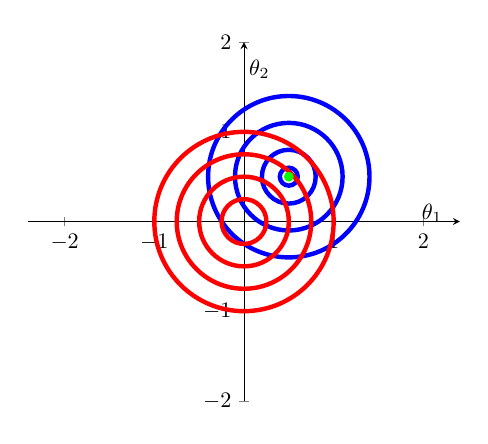
\begin{tikzpicture}[scale=0.8]
        \begin{axis}[
         axis lines=middle,
                axis equal,
         xmin=-2, xmax=2, ymin=-2, ymax=2,
         every axis x label/.style={at={(current axis.right of origin)},anchor=west,above=2em,right=1.5em},
         every axis y label/.style={at={(current axis.north)},above=2em,right=1.5em},
        xlabel = $\theta_1$,
        ylabel = $\theta_2$
        ]
        \draw [blue, line width=2pt](axis cs: 0.5, 0.5) circle [radius=0.1];
        \draw [blue, line width=2pt](axis cs: 0.5, 0.5) circle [radius=0.3];
        \draw [blue, line width=2pt](axis cs: 0.5, 0.5) circle [radius=0.6];
        \draw [blue, line width=2pt](axis cs: 0.5, 0.5) circle [radius=0.9];

        \draw [red, line width=2pt](axis cs: 0, 0) circle [radius=1];
        \draw [red, line width=2pt](axis cs: 0, 0) circle [radius=0.75];
        \draw [red, line width=2pt](axis cs: 0, 0) circle [radius=0.5];
        \draw [red, line width=2pt](axis cs: 0, 0) circle [radius=0.25];
        \addplot[green,only marks] coordinates{(0.5, 0.5)};
        \end{axis}
    \end{tikzpicture}
            
            }
    \subfigure[函数最优解落在可行域之外]{
    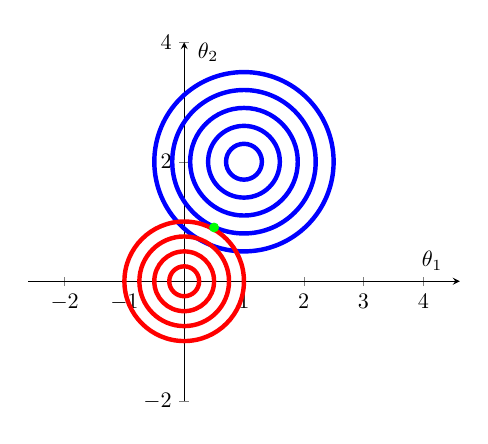
\begin{tikzpicture}[scale=0.8]
    \begin{axis}[
        axis equal,
         axis lines=middle,
         xmin=-2, xmax=4, ymin=-2, ymax=4,
        xlabel = $\theta_1$,
        ylabel = $\theta_2$,
        every axis x label/.style={at={(current axis.right of origin)},anchor=west,above=2em,right=1.5em},
         every axis y label/.style={at={(current axis.north)},above=2em},
        ]
        \draw [blue, line width=2pt](axis cs: 1, 2) circle [radius=0.3];
        \draw [blue, line width=2pt](axis cs: 1, 2) circle [radius=0.6];
        \draw [blue, line width=2pt](axis cs: 1, 2) circle [radius=0.9];
        \draw [blue, line width=2pt](axis cs: 1, 2) circle [radius=1.2];
        \draw [blue, line width=2pt](axis cs: 1, 2) circle [radius=1.5];

        \draw [red, line width=2pt](axis cs: 0, 0) circle [radius=1];
        \draw [red, line width=2pt](axis cs: 0, 0) circle [radius=0.75];
        \draw [red, line width=2pt](axis cs: 0, 0) circle [radius=0.5];
        \draw [red, line width=2pt](axis cs: 0, 0) circle [radius=0.25];
        \addplot[green, only marks] coordinates{(0.5, 0.9)};

    \end{axis}
	\end{tikzpicture}
            }
          
\caption{不等式约束下的极值问题\label{fig:L2_lang}}
\end{figure}


对于图\ref{fig:L2_lang}(a)中最优解落在可行域的情况,二范数正则并不影响参数估计的结果,此时参数估计依然是无偏的。但实际场景中往往是图\ref{fig:L2_lang}(b)中的情况,即最优解落在可行之外的情况,此时参数估计是有偏的,并且,由于约束条件下的极值为目标函数于可行域的切面,而可行域是以原点为球心,以微小量为半径的超球体,这将使得参数最终的估计值是一个较小的值,为了进一步说明这个现象,我们不妨对式\ref{equ:mse_l2_loss}中的准则函数进行求导
\begin{equation}
\begin{split}
	\frac{\partial L(\theta)}{\partial \theta} &= \frac{\partial(X\theta  - Y)^2}{\partial \theta} + 2\alpha \theta\\
	&= \nabla_{MSE} + 2\alpha \theta
\end{split}
\end{equation}
当使用梯度下降进行训练是,参数的更新方式为
\begin{equation}
	\theta := \theta -\eta (\nabla_{\theta} + 2\alpha \theta)
\end{equation}
其中,$\eta$是学习率,由于$\alpha$是超参数,当其选取为
\begin{equation}
	\alpha = \frac{1 - \eta}{2\eta}
\end{equation}
则有
\begin{equation}
\begin{split}
	\theta &:= \theta -\eta (\nabla_{\theta} + \frac{1-\eta}{\eta} \theta)\\
	&= \theta - \eta\nabla_{\theta} - (1-\eta)\theta\\
	&=\eta(\theta - \nabla_{\theta})
 \end{split}
\end{equation}
这其实等价于两个参数更新过程,首先执行梯度更新,即$\theta - \nabla_{\theta}$,然后在将更新后的参数按$\eta$进行缩小,这种技术也被称为权衰减,所以我们说,权衰减等价于L2正则。

如果从罚函数的观点看L2正则,那么对于罚函数$\theta\theta^T$而言,当$\theta$较大时,惩罚项也较大,当$\theta$趋于0时,惩罚项趋于0,但此时梯度$\theta$也相应地趋于0,因此$\nabla_{\theta}$在这时候成为主导地位,所以$\theta$很难收敛到0,除非正则的权重设置得很大。

接下来我们讨论一下为什么加了L2正则的线性回归被称为岭回归。对于目标函数\ref{equ:mse_l2_loss},其极值所在点为导数为0处,即
\begin{equation}
	2X^T(\theta X - Y) + 2\alpha\theta = 0
\end{equation}
则
\begin{equation}
	\theta = (X^TX + \alpha I)^{-1}X^TY
\end{equation}
可以看到,这个结果于式\ref{equ:linear_regress_approx_solve}是等价的。由于$X^TX + \alpha I$存在一个微小量$\alpha I$,所以它的逆是必定存在的,不需要考虑不可逆的问题,同时,正是因为在$X^TX$的对角线上加了这个微小量,值增高了它的“岭”,所以称为岭回归或脊回归。 另一方面,正如我们在图\ref{fig:L2_lang}中看到的,加入了L2范数正则后,参数估计不再保证无偏性。

我们从贝叶斯的角度来讨论一下L2正则,现在,模型的参数$\theta$不再认为是客观存在但未知的变量,而是一个概率分布,这也是贝叶斯学派和经典学派的分歧点,即,模型的参数是客观存在的,还是一个概率分布。我们假设,$\theta$服从一个均值为0,方差恒定的高斯分布,即
\begin{equation}
	\theta \sim \mathcal{N}(0, \sigma_\theta^2)
\end{equation}




% subsection ridge_回归 (end)






\subsection{Lasso 回归} % (fold)
\label{sub:lasso_回归}

% subsection lasso_回归 (end)



\subsection{ElasticNet} % (fold)
\label{sub:elasticnet}

% subsection elasticnet (end)

\subsection{多项式回归} % (fold)
\label{sub:多项式回归}

% subsection 多项式回归 (end)

% section 线性回归及其正则 (end)

\section{指数族与广义线性模型} % (fold)
\label{sec:指数族与广义线性模型}
\subsection{指数族} % (fold)
\label{sub:指数族}

% subsection 指数族 (end)
\subsection{对数几率回归} % (fold)
\label{sub:对数几率回归}

% subsection 对数几率回归 (end)

\subsection{Softmax 回归} % (fold)
\label{sub:softmax_回归}

% subsection softmax_回归 (end)

\subsection{泊松回归} % (fold)
\label{sub:泊松回归}

% subsection 泊松回归 (end)

% section 指数族与广义线性模型 (end)

\section{贝叶斯方法} % (fold)
\label{sec:贝叶斯方法}

\subsection{贝叶斯回归} % (fold)
\label{sub:贝叶斯回归}

% subsection 贝叶斯回归 (end)

\subsection{朴素贝叶斯} % (fold)
\label{sub:朴素贝叶斯}

% subsection 朴素贝叶斯 (end)


% section 贝叶斯方法 (end)



\section{支撑向量机} % (fold)
\label{sec:支撑向量机}

% section 支撑向量机 (end)


% chapter 线性模型 (end)